\documentclass[]{msulabm}
\usepackage[utf8]{inputenc}
\usepackage{amsmath}
\usepackage{graphicx}
%\usepackage[linktocpage]{hyperref}  % if not using colorlinks, use linktocpage
\usepackage[colorlinks]{hyperref}  % if not using colorlinks, use linktocpage
\usepackage{bm}            % bold math
\usepackage{multirow}
\usepackage[table]{xcolor} % provide alternating rows with colors
\usepackage{textcomp}
\usepackage{xfrac} % gives split-level fractions with '\sfrac{a}{b}
\usepackage{multicol}
\usepackage[section]{placeins} % provides \FloatBarrier, to keep floats from crossing this barrier
\usepackage{amssymb}
\usepackage{wrapfig} % provides wrapping figures with text.
%\usepackage{enumitem} % gives \begin{enumerate}[resume] to resume counting from previous enumerate
%\usepackage{subfigure}
%\usepackage{tikz} % to draw arrows
\usepackage{xtab} % provides xtabular, tabular environment that spans multiple pages and other awesome things
\usepackage[style=phys,biblabel=brackets,pageranges=false]{biblatex}
\usepackage{pdflscape}
\usepackage{ragged2e}
\usepackage{longtable}
\usepackage{mathabx} % gives astronomy symbols like \Earth
\usepackage{pdfpages}

\bibliography{references-manual,bbarker-zotero}

\newcommand{\abs}[1]{\left\lvert#1\right\rvert}

\title{Laboratory Manual}
\author{ASTR 24100 Physics of Stars \\ \\ The University of Chicago}
\date{Winter 2023}

\pagestyle{ruled}

\definecolor{lgray}{rgb}{.2,.2,.2}

\makeevenfoot{ruled}{\thepage}{\footnotesize{\textit{Last updated \today}}}{}
%\makeevenfoot{ruled}{\thepage}{}}{}
\makeoddfoot{ruled}{}{\color{lgray} \tiny{This work is licensed under \href{http://creativecommons.org/licenses/by-sa/4.0/}{CC BY-SA 4.0} by \href{mailto:bbarker@uchicago.edu}{the University of Chicago}.}}{\thepage}


% allows us to use subcaptions from the memoir class in figures. See Memoir Section 10.9
\newsubfloat{figure}

% don't worry so much about filling every page.
%\raggedbottom

% raise the penalty for splitting footnotes across different pages. Default is 100.
\interfootnotelinepenalty=10000

%\includeonly{amplifier/amplifier} 

% creates a standard length to use 
\newlength{\answerskip}
%\setlength{\answerskip}{90pt} 

%% use plus / minus if latex is squeezing the answer space too much
\setlength{\answerskip}{2cm plus 0.2cm minus 0.2cm}

\newlength{\qaskip}
\setlength{\qaskip}{\answerskip}
\addtolength{\qaskip}{\baselineskip}

% reduce vertical space between chapters in table of contents. Default is 2em.
\setlength{\cftbeforechapterskip}{1em}

% allow for extra line on a page to help prevent widow/orphan lines.
\sloppybottom

% Now we can caption a table outside of the table float environment (good for multi-page tables)
\newfixedcaption{\freetabcaption}{table}

%\includeonly{snells-law/snells-law}
%\includeonly{ohms-law/ohms-law}

\begin{document}
\maxtocdepth{chapter}

 % start roman numbering
 \frontmatter

\maketitle

%\clearpage

%Brent W. Barker

%Department of Astronomy \& Astrophysics

%The University of Chicago

%5640 South Ellis Ave.

%Chicago, IL 60637

%\href{mailto:bbarker@uchicago.edu}{bbarker@uchicago.edu}

%\vspace{2\baselineskip}

%\includegraphics{cc-by-sa-88x31}

%\textcopyright{} 2018 Brent W. Barker. Except where otherwise noted, this work is copyrighted under the Creative Commons Attribution-ShareAlike International 4.0 License. To view a copy of this license, visit \url{http://creativecommons.org/licenses/by-sa/4.0/}.

%\vspace{\baselineskip}

%These labs, excluding "Impulse and Momentum" and the appendices, are a derivative of "\href{https://%sites.google.com/site/scientificabilities/ISLE-labs}{ISLE Labs}" by the Rutgers Physics and Astronomy %Education Research group, used under the Creative Commons Attribution International 4.0 License.
%To view a copy of this license, visit \url{http://creativecommons.org/licenses/by/4.0/}.

%At Rutgers University, many people contributed to this project over the years.
%The list of names is very long and includes: Eugenia Etkina, Alan Van Heuvelen, Suzanne Brahmia, David %Brookes, Michael Gentile, Anna Karelina, Michael Lawrence, Marina Milner-Bolotin, Sahana Murthy, Maria %Ruibal-Villasenor, Aaron Warren, Xueli Zou.

 % skip to next right leaf (``recto'')
 \cleartorecto

 % the star means that the ToC itself is not listed in the ToC
 \tableofcontents*

 % start arabic numbering
\mainmatter 

%\chapter{Spectrum of black body radiation}

%\includepdf[pages={1-12}]{blackbody-pos/lab-black-body}

\chapter{Inventing Color}\footnote{Contributions from Brent Barker, Mike Gladders, Amanda Pagul, and others.}

%todo for in-person lab: subtraction of colors for filter part does not work. magnitudes are already logarithmic, so it works for them. Try doing measurements and using ratio of g/r instead of difference, adjust lab accordingly.

%TODO rewrite rgb image directions. these are very unclear.

%TODO for "conduct an experiment", be more clear about what deliverables / product is wanted

Everything glows (gives off electromagnetic radiation) when it has a temperature --- particles are wiggling around randomly (faster if it's hotter) and giving off energy as they wiggle. This \textbf{thermal radiation}, also called blackbody radiation, is the same for any object at the same temperature. The spectral density $B$ of this radiation at wavelength $\lambda$ and temperature $T$ is given by Planck's Law:
\begin{equation}\label{ic:eq:planck}
 B(\lambda, T) = \frac{2 h c^2}{\lambda^5}
 \frac{1}{\exp\left( \frac{hc}{\lambda k_\textrm{B} T} \right) - 1} \,,
\end{equation}
where $h$ is the Planck constant, $c$ is the speed of light in the medium, and $k_\textrm{B}$ is the Boltzmann constant. The peak of this distribution $\lambda_\textrm{peak}$ is given by Wien's displacement law,
\begin{equation}\label{ic:eq:wien}
	\lambda_\textrm{peak} = \frac{b}{T} \,,
\end{equation}
where $b \approx 2898\:\mu$m$\cdot$K is Wien's displacement constant. This universal behavior means we can take something's temperature by looking at the spectrum of light it gives off. This is great for learning about something's temperature at a distance, like stars.

%Incandescent lightbulbs are so warm that they glow in the visible spectrum (like stars). In this lab, you'll investigate the radiation that is given off by a lightbulb at various temperatures, then use filters to mimic the situation astronomers are in when they observe astronomical objects with different color filters. You'll invent a metric to numerically state the temperature of the lightbulb, even without knowing the actual temperature. Finally, you'll use the various images that you took with SEO with different color filters and combine them to form a color image.

\subsection{Team roles}

\begin{steps}
	\item \textbf{Decide on roles} for each group member.
\end{steps}

The available roles are:
\begin{itemize}
	\item Facilitator: ensures time and group focus are efficiently used
	\item Scribe: ensures work is recorded
	\item Technician: oversees apparatus assembly, usage
	\item Skeptic: ensures group is questioning itself
\end{itemize}

These roles can rotate each lab, and you will report at the end of the lab report on how it went for each role. Some members will be holding more than one role. For example, you could have the skeptic double with another role. Consider taking on a role you are less comfortable with, to gain experience and more comfort in that role.

Additionally, if you are finding the lab roles more restrictive than helpful, you can decide to co-hold some or all roles, or think of them more like functions that every team needs to carry out, and then reflect on how the team executed each function.

%\subsection{Add members to Canvas lab report assignment group}
%
%\begin{steps}
%	\item On Canvas, navigate to the People section, then to the ``Groups'' tab. Scroll to a group called ``L3 Inventing Color [number]'' that isn't used, and have each person in your group add themselves to that same lab group.
%\end{steps}
%
%This enables group grading of your lab report. Only one person will submit the group report, and all members of the group will receive the grade and have access to view the graded assignment.

\section{Exploring thermal radiation}\label{ic:sec:exploring}

\begin{steps}
	\item\label{ic:step:load-sim} Load the interactive thermal radiation simulation at \url{https://phet.colorado.edu/sims/html/blackbody-spectrum/latest/blackbody-spectrum_en.html}
	
	\item Play with the controls and see what happens. Discuss among your team.
	
	\item Find a pattern --- how does the shape change as the temperature goes up? For example, how does the peak wavelength change, and how about the total radiated power (area under curve)? \textbf{Record your observations.}
	
	\item At what peak wavelength do you radiate? Use the sim to determine this and estimate your uncertainty. \textbf{Record your findings.}
	
	\item Using your estimated temperature, calculate your peak wavelength according to Wien's law.
	
	\item\label{ic:step:qual-color} Comparing the spectra of the light bulb, Sun, and Sirius A, how can you use the spectrum to determine what color each one appears as?
\end{steps}

\section{CCDs and filters}

Cameras have come a long way since the days of developing film, but sensors are not as smart you might think. They register light, but they can't usually tell the color (i.e. wavelength) of the incoming photons. So then how do you get a color image? In astronomy (and in your cell phone!) color images are generated by measuring the amount of light at specific colors and then combining these measurements to create a colorful image. A filter is used to select bands of color to allow through. In consumer cameras and phone cameras, these filters are permanently attached to the front of individual pixels. In astronomical imaging, there is no permanent filter, and different filters are moved into place.

\subsection{Filters}
Light is composed of photons with energies that determine their wavelengths (shorter wavelength $\implies$ higher energy). Thus every light source exhibits a \textbf{spectrum} of energies based on its energetic components, determined by the physics of the light emission process. Thus, observing the energetic constituents of light from astronomical objects - a.k.a. observing the spectrum of emitted radiation - is a fundamental tool in observational astrophysics. However, obtaining the specific intensity of radiation as a function of energy from an astronomical source is challenging. An easier way to asses the electromagnetic energies observed is to image them in different filters: materials that are transparent to a known range of wavelengths and opaque to all others. Thus, one can image the same object with multiple different filters to get a sense of the wavelength regimes that make the strongest contributions to the overall electromagnetic output.

A filter is characterized by its \textbf{transmission function}: a function that characterizes the amount of light that is transmitted by the filter at each wavelength. Figure~\ref{sot:fig:filters} shows the transmission functions for standard astronomical filters that are used in the Sloan Digital Sky Survey and now used as standard filters elsewhere.% (similar to the ones you'll be using in this class).

\begin{figure}
	\centering
	\includegraphics{small-optical-telescopes/fig_sdss_filters_1.png}
	\caption{Filter Transmission Functions for the Sloan Digital Sky Survey, overlaid on a stellar spectrum (in this case the spectrum is probably an
		A-type star). The magnitude observed by each filter will be proportional to the integrated spectrum multiplied by the filter transmission. It's clear in this image that the underlying spectrum of the star will cause the different filters to have different magnitudes. How would these magnitudes change if the spectrum was, say, of an M-star instead? (Image source: \url{http://www.astroml.org/\_images/fig\_sdss\_filters\_1.png})}\label{sot:fig:filters}
\end{figure}

\begin{steps}
	\item Open the Google Sheet found here: \url{https://docs.google.com/spreadsheets/d/1qgTqiqWOFCzYuSmHeT-5hwy_lBYO0Tvu24kM955nfq4/edit?usp=sharing}
	
	\item Make a copy of this sheet for your group to use.
\end{steps}

This spreadsheet calculates the same theoretical thermal radiation curve (according to Planck's Law) as the PhET simulation above, seen in the first two columns. Then it applies the transmission functions of the SDSS filters and plots the remaining power spectrum that gets through each filter. Finally, it sums up each filter's power spectrum and gives a total pixel value and magnitude. The pixel value is the relative number of counts a pixel with that filter would read. This is proportional to the brightness it sees.

\subsection{Magnitude}

Astronomers measure brightness of stars using a measurement system called \textit{magnitude}. About two millenia ago, astronomers categorized stars into 6 different brightness classes, 1st class through 6th class. When brightness began to be more quantified, it was found that first magnitude stars were about 100 times brighter than 6th magnitude stars. Then it was decided to scale the 6 classes logarithmically, to account for the several orders of magnitude involved. The relationship between intensity (power per unit area) \textit{I} and magnitude $m$ is defined as
\begin{equation}
 m \equiv -2.5 \log_{10} \left(\frac{I}{I_\textrm{ref}}\right) \,,
\end{equation}
where $I_\textrm{ref}$ is the intensity of some standard reference object. In the spreadsheet, these values marked as magnitudes are not technically magnitudes, since we are not using the dimensions of intensity, but it will help your analysis to treat them as such.

\subsection{Color index}

In Section \ref{ic:sec:exploring}, you learned that the color of a thermally radiating object is related to its temperature. Here, you will develop a quantitative color index and use it to determine the temperature of the Sun.

\begin{steps}
	\item\label{ic:step:see-thermal} In the spreadsheet, change the temperature of the blackbody (edit cell \texttt{B1}) and watch how the spectrum changes, and how the filter magnitudes change with respect to each other. \textbf{Record your observations.}
\end{steps}
	
The magnitude depends not just on the temperature, but also on the size of the star and the distance away from us. So to characterize a star's color quantitatively, independent of the size and distance, astronomers use a ratio of brightnesses of different filters. This is equivalent to subtracting the magnitudes. The subtraction of two broadband filter magnitudes is called the \textit{color index}.

\subsection{Correlating color index and temperature}

In order to use the color index of a star to find its temperature, you need to determine how the two related to each other. If you assume the EM radiation emitted by the star is entirely due to thermal radiation, then you can find the theoretical color index of a blackbody at various temperatures, and then find where the star's color index sits on that graph.

\begin{steps}
	\item Choose the filters from which to make your color index. Do you want to choose filters that detect wavelengths right next to each other, or farther apart? If you're not sure, try both and see which is better for this application. You can call the resulting color index ``$x - y$'', for example $g' - r'$ if you are subtracting the $r'$ filter value from the $g'$ value.
	
	\item\label{ic:step:tempcolor} Make a table and graph of temperature vs. color index. \textbf{Record your table and graph.}
\end{steps}

\subsection{Taking the Sun's temperature}

\begin{steps}
	\item Switch to the ``Sun'' tab in the spreadsheet. This has experimentally determined values for the intensity of EM radiation impinging on the Earth from the Sun, alongside the same filtering system as in the theoretical tab.
	
	\item\label{ic:step:proc-color} Design a procedure to use the filter magnitudes of the Sun to determine its temperature and your uncertainty of that temperature. Run this procedure by your TA to get feedback on it before starting.
	
	\item Conduct your experiment and keep a log.
	
	\item Look up the effective temperature of the Sun's photosphere on Wikipedia.
	
	\item Calculate the percent difference between your value and the one that Wikipedia references:
	\begin{equation}
	 \textrm{percent difference} = \frac{\abs{a-b}}{\frac{a+b}{2}} \times 100\%
	\end{equation}
	
	\item\label{ic:step:solar-compare} Use the $t'$ statistic described in Appendix\ \ref{unc:sec:comparing} to compare the two values and interpret the result --- do these two measurements really measure the same thing? If they are very different, check your procedure, and if the difference stays, discuss what could be different about the methods used to find the temperature, or different assumptions used. \textbf{Record your discussion.}
\end{steps}

%\section{Lightbulbs}
%
%Light can be made of many different wavelengths at the same time. It combines to form a color that we perceive. To see what colors make up light, we can split them again with a triangular prism, or with a \textit{diffraction grating}.
%
%\begin{steps}
%	\item Use the diffraction grating to view the lightbulb while the lightbulb is at full voltage (120 V). Hold up the grating in front of your eye, with the text on the frame upright. Start by looking at the lightbulb through it, then turn your feet to the left or right about 30 degrees, letting your whole body-arm-grating system rotate with your feet. You should see a rainbow. This is all the colors that make up the light coming from the lightbulb, split into different wavelengths.
%\end{steps}
%
%\subsection{Orientation to the digital spectrometer}
%
%\begin{framed}
%	\textbf{Warning! Fragile Equipment!} If the fiber optic cable is bent into a circle of less than 9 cm (6 inch) diameter, then the fiber inside may break.
%	
%	Also, the blue end cap should be replaced on the end of the fiber optic cable when you are done using it, to protect from dust and debris entering.
%\end{framed}
%
%A digital spectrometer also uses a diffraction grating, but instead of collecting the dispersed light on a screen to be viewed by people, it collects the light with a charge-coupled device (CCD), an array of light-sensitive pixels much like a digital camera. It then translates the position on the CCD to individual wavelengths and displays a plot of intensity vs. wavelength on a computer. %TODO (see Figure~???)
%Another difference is that we use an optical fiber to collect the light.
%
%Here are a few guidelines:
%\begin{itemize}
%	
%	\item \textbf{Background subtraction.} When you are observing the spectrum of something, there may be stray light entering that is not coming from the thing you are studying. To remove this \textit{background} from the plot, select the gray lightbulb icon in the toolbar. This records the current plot as the background. To display the plot while subtracting the background, select the icon with the minus-lightbulb. To go back to viewing the full spectrum including the background, select the blue S icon.
%
%	\item \textbf{Oversaturation}. If, when you zoom out all the way, the plot includes a flat line near the top of the plot, this means that the pixels of the image sensor are recording their maximum value, and they cannot tell you the actual intensity. Reduce the intensity by either reducing the integration time (upper-left corner) or moving the fiber optic cable off-center, so that it receives less light. Note that if you change either of these, then the background frame is no longer correct and must be remeasured.
%
%	\item \textbf{Low signal}. If the target is dim, then you might find when you zoom in, the plot is not smooth, but instead jagged and hard to find patterns in. In this case, increase the integration time using the field in the upper-left of the program window. This increases the exposure time, equivalently. Note that if you change the integration time, then the background frame is no longer correct and must be remeasured.
%
%	\item \textbf{Saving data.}
%	
%	\begin{itemize}
%		\item Save the images of spectra and numeric files that you generated with SpectraSuite
%	during your experiments on a USB stick, so that you can use them at home during
%	preparation of your report (you can also email them as attachments from your
%	computer at the end of the lab).
%	
%	\item You should open a word processor document and a spreadsheet document in which you can save your measured
%	spectra at the beginning of your work. To save an image of your graph, click on
%	the fourth icon from the left in the Spectrum IO controls. %TODO (Fig.~???)
%	This will copy
%	an image of the graph to the clipboard. Then in your word processor, paste the image by pressing
%	Ctrl-V.
%	
%	\item To save spectrum in the digital form, click on the third from the left icon in
%	Spectrum IO controls (to the right of print icon). This copies it to clipboard. In
%	Excel file make sure you are in a new sheet and press Ctrl-V. This should create
%	to columns of numbers: wavelength (in nm) and counts for your spectrum.
%	
%	\item An alternative way to save the data is to click on the floppy disk icon in the
%	Spectrum IO controls. The format must be ``Tab delimiter, no header''. The
%	writing directory must be specified (``Browse'' button). The spectrum is saved in a
%	text file (.txt) as two columns, the first column giving the wavelength in nm, the
%	second column the corresponding intensity. This file can be imported into a spreadsheet or plotting program.
%	\end{itemize}
%\end{itemize}
%
%\subsection{Observing a lightbulb}
%
%\begin{steps}
%	
%	\item Using the spectrometer, observe the spectrum created by a lightbulb at various brightnesses / voltages.  What's the overall shape? \textbf{Record your answer.}
%	
%	\item How does the shape change when the brightness increases? \textbf{Record your answer.}
%	
%	\item How does the peak frequency change? \textbf{Record your answer.}
%	
%	\item How does the visual color of the bulb change as it gets brighter? \textbf{Record your answer.}
%	
%	\item\label{ic:step:pattern} As the lightbulb gets brighter, the filament inside gets hotter --- the temperature increases. If all objects act like the tungsten filament as it gets hotter, what general pattern can you state about the light given off by an object as a function of its temperature? \textbf{Record your answer.}
%
%\end{steps}
%
%Cameras have come a long way since the days of developing film, but sensors are not as smart you might think. They register light, but they can't usually tell the color (i.e. wavelength) of the incoming photons. So then how do you get a color image? In astronomy (and in your cell phone!) color images are generated by measuring the amount of light at specific colors and then combining these measurements to create a colorful image. A filter is used to select bands of color to allow through. In consumer cameras and phone cameras, these filters are permanently attached to the front of individual pixels. In astronomical imaging, there is no permanent filter, and different filters are moved into place.
%
%\begin{steps}
%	\item View the lightbulb's spectrum with the diffraction grating again, this time alternately holding the red and green filters between the grating and the bulb. Observe and \textbf{record} the effect of the filter on the spectrum.
%	
%	\item Use the red and green filters in front of the fiber optic input to the spectrometer to see how they affect the spectrum that is received. \textbf{Save a graph of the spectrum with each filter and include in your report.}
%\end{steps}
%
%In a regular astronomical image, each pixel gives just one value --- the number of counts detected in that pixel, regardless of the wavelength of the photon detected. We can treat the fiber optic as a single-pixel camera if we count up the total number of counts detected. To find that total number, you can find the area under the curve in the plot.
%
%\begin{steps}
%	\item With no filter, add up the total number of counts detected by calculating the area under the curve. To do this in an approximate way, count the number of boxes underneath the curve, then multiply this by the height of one box (in counts per nanometer) and by the width of one box (in nanometers). \textbf{Record this value.}
%	
%	\item Do the same for the spectrum using the red and green filters separately. Note that the values are different for different filters. This difference (for example, the green value minus the red value) can tell us a quantitative number for what color this object is. \textbf{Record the red, green, and $g-r$ values.}
%\end{steps}
%
%Now you have the value of our single-pixel camera for the case of clear (no filter), red, and green filters. Time to revisit the pattern found above in Step \ref{ic:step:pattern}.
%
%\begin{steps}
%	\item If that pattern from Step \ref{ic:step:pattern} is true, what should happen to the relative values of red and green as the voltage is increased? Should one increase more than the other? What should happen to the quantitative color $g-r$? \textbf{Record your answers.}
%	
%	\item Perform an experiment to test whether this prediction is supported. \textbf{Record your procedure, analysis, and results.}
%\end{steps}

\section{Creating a color image}

To create the beautiful color astronomy images we like to see, one must manually combine images taken with different filters. There are always choices to be made that will change how the combined image looks.

\begin{steps}
	\item\label{ic:step:color-image} Using the directions below, create a false color image of either the Orion nebula (M42), a stellar nursery, or the Crab nebula (M1), the remnant of a supernova. You can find the relevant images on Canvas in the Lab module.
\end{steps}

Now you'll create a color image from three separate images of the same target. You can use the broadband filters that you used in the previous section, and you can also try using the narrowband filters h-alpha, oiii, and sii. These filters only allow specific wavelengths through, that correspond to particular electronic excitations of hydrogen, oxygen, and silicon, respectively. Different features can be seen with different filters, as seen in Figure \ref{ic:fig:m1-filters}.

\begin{figure}
	\centering
	\includegraphics[width=\textwidth]{inventing-color/m1-different-filters-lores.png}
	\caption{Images of M1, the Crab Nebula, in different wavelength filters, revealing different features. Top row from left to right are the narrowband h-alpha, oiii, and sii filters. Bottom row is the broadband g', r', and i'. The structure comes out nicely in the narrowband, while there are more stars in broadband.}\label{ic:fig:m1-filters}
\end{figure}

Since there is not a 1-to-1 correspondence between the red-green-blue options in DS9 and the filters available, you will assign a different, arbitrary filter to each color in DS9. This makes the image a \textit{false color image}, since the colors we will see in it do not correspond to the actual wavelength of the light captured.

\textbf{Loading and manipulating images in ds9 consists of:}
\begin{itemize}
\item loading an image  (file $>$ open)
\item setting lower, upper limits (z1,z2) on an image  (scale $>$ various algorithms; use scale $>$ scale parameters for full control). See Figures \ref{ic:fig:z-min-max}--\ref{ic:fig:z-small} for examples.
\item controlling the intensity mapping within those bounds (mouse right click-and-hold and drag)
\end{itemize}

\begin{figure}
	\includegraphics[width=0.5\textwidth]{inventing-color/z-min-max}
	\includegraphics[width=0.5\textwidth]{inventing-color/z-mid}
	\caption{Proper choice of data ranges is important. The default for ds9 is often the min/max values in the image, which can be a poor choice if there are outlier pixels, as shown here on the left. The red line shows the lower limit z1, which is mapped to no color (black here), and the green line is the upper limit z2, mapped to full color (white here). Pixel values between these are shown in various brightnesses of the color. On the right, z1 and z2 are more tuned to the distribution of pixel values, which more effectively uses the dynamic range of the display for pixel values where there are significant amounts of data.}\label{ic:fig:z-min-max}
\end{figure}

\begin{figure}
		\includegraphics[width=0.5\textwidth]{inventing-color/z-small}
		\caption{Smaller values of z2 will emphasize fainter values in the target. Compare the image to the left to the right-hand image above.}\label{ic:fig:z-small}
\end{figure}

\textbf{You can change the zoom and center location in an image by} 
\begin{itemize}
\item moving around in image (mouse middle click if edit$>$point is set[the default], or edit$>$pan and mouse left click)
\item zooming in and out (mouse wheel, zoom$>$ +,- etc.)
\end{itemize}

\textbf{To build a color image}
\begin{itemize}
	\item Identify and download from SEO your three different filter image FITS files.
\item Open a color (rather than monochrome) frame:  Frame $>$ new rgb
\item Open the red, green, infrared files using the rgb subwindow to select which channel you are working in, and then scale and control intensities on each one. 
\item There are many possible ways to scale the images. Some testing suggests that choosing Scale $>$ ASINH (or Linear or Square Root as other choices) and Scale $>$ 99.5\% (or maybe 99\% or 98\%)  produces reasonable results. Experiment!
\item One thing to note: the rgb subwindow allows you to control how the images are aligned spatially via the “align” menu at the top. There are three relevant choices: “WCS”, “Image” or “Physical”.  The latter two should give the same result in this instance. “WCS” alignment uses information in the image header that has been added by the processing pipeline, that establishes a World Coordinate System (this tells ds9 and other programs how pixel x,y values are mapped into the sky coordinates - typically Right Ascension [east/west] and Declination [north/south]). The default is WCS and should work fine, if the images processed correctly. If that doesn’t look good, you could try the others. If that still doesn’t look good, note that you tried your best, and give an example of how it didn’t work will in either mode. Examples of good and bad image alignment are shown in Figure \ref{ic:fig:rgb-bad}.
\end{itemize}

\begin{figure}
	\includegraphics[width=0.5\textwidth]{inventing-color/rgb-bad}
	\includegraphics[width=0.5\textwidth]{inventing-color/rgb-good}
	\caption{Zoom-in on a color image, showing poor (left) and good (right) image alignment across filters. Note how objects are shifted between different color channels in the poorly aligned image.}\label{ic:fig:rgb-bad}
\end{figure}

\section{Report checklist and grading}

Each item below is worth 10 points. See Appendix\ \ref{cha:lab-report-format} for guidance on writing the report and formatting tables and graphs.

\begin{enumerate}

	\item List of team role assignments and agreements about group communication

	\item Pattern of how shape of spectrum changes with temperature, your peak wavelength, and how to use spectrum to predict color (Steps \ref{ic:step:load-sim}--\ref{ic:step:qual-color}).
	
	\item Observations of how spectrum and filter magnitudes change with temperature (Step \ref{ic:step:see-thermal}).
	
	\item Table and graph of color index versus temperature (Step \ref{ic:step:tempcolor}).
	
	\item Procedure, calculations, and determination of solar temperature and uncertainty.
	
	\item Comparison with percent difference, $t'$ statistic, and discussion (Steps \ref{ic:step:proc-color}--\ref{ic:step:solar-compare}).
	
	\item Your beautiful color image (Step \ref{ic:step:color-image}).
	
	\item Discuss the findings and reflect deeply on the quality and importance of the findings. This can
	be both in the frame of a scientist conducting the experiment (“What did the experiment tell us
	about the world?”) and in the frame of a student (“What skills or mindsets did I learn?”).
	
%	\item A 100–200 word reflection on group dynamics and feedback on the lab manual. Address the
%	following topics: who did what in the lab, how did you work together, what successes and
%	challenges in group functioning did you have, and what would you keep and change about the
%	lab write-up?
	
	\item Write a 100--200 word paragraph reporting back from each of the four roles: facilitator, scribe, technician, skeptic. Where did you see each function happening during this lab, and where did you see gaps? What successes and challenges in group functioning did you have? What do you want to do differently next time?
\end{enumerate}

%\chapter{Using light waves to measure small distance changes (Michelson interferometer)}

\section{Introduction}

With the basic properties of waves and wave interference established (via the ripple tank) and the same behavior
demonstrated in light (via the laser-based modern version of Young's double slit experiment) we are now finally ready to
look at a Michelson interferometer. This technology is the basis of the LIGO experiment. You may want to refer back to
the introduction of Lab~\ref{cha:ripple-tank} to remind yourself of some details. LIGO itself is a large experiment that has
been constructed over several decades of work and technology development, and so is many orders of magnitude more
precise and sensitive than what we can do in an hour on a lab bench. Nevertheless, the basic principles are the same.

%\section{Learning Goals}

\section{Team roles}

\begin{steps}
	\item \textbf{Decide on roles} for each group member.
\end{steps}

The available roles are:

\begin{itemize}
	\item Facilitator: ensures time and group focus are efficiently used
	\item Scribe: ensures work is recorded
	\item Technician: oversees apparatus assembly, usage
	\item Skeptic: ensures group is questioning itself
\end{itemize}

These roles can rotate each lab, and you will report at the end of the lab report on how it went for each role. If you have fewer than 4 people in your group, then some members will be holding more than one role. For example, you could have the skeptic double with another role. Consider taking on a role you are less comfortable with, to gain experience and more comfort in that role.

Additionally, if you are finding the lab roles more restrictive than helpful, you can decide to co-hold some or all roles, or think of them more like functions that every team needs to carry out, and then reflecting on how the team executed each function.

\section{Add members to Canvas lab report assignment group}

\begin{steps}
	\item On Canvas, navigate to the People section, then to the ``Lab 3 Groups'' tab. Find a group that is not yet used, and have each person in your group add themselves to that same lab group.
\end{steps}

This enables group grading of your lab report. Only one person will submit the group report, and all members of the group will receive the grade and have access to view the graded assignment.

\section{Observation experiment: demonstration of the interferometer}

\subsection{Goal}

Observe the flow of light in the Michelson interferometer simulation.

\subsection{Available equipment}

\begin{itemize}
	\item A virtual Michelson interferometer found at \url{https://www.geogebra.org/m/msfpudej}
	\begin{itemize}
		\item Note: in the sim, do not zoom in and out by scrolling --- when this happens, the coordinate system appears to shrink and expand, leading to the mirrors seeming to move in space.
	\end{itemize}
\end{itemize}

\subsection{Rubrics to be assessed for this section}

None.

\section{Steps}

\begin{steps}
	\item Load the virtual apparatus at the address listed in the available equipment section.
	
	\item Click the refresh button in the simulation, to the right of the Zeit slider. This fixes a bug where the green wave does not fully display.

	\item Slide Zeit (German for "time") to the left to equal 0. Uncheck "Weg Spiegel 1" (wave path 1)
\end{steps}

This is the Michelson interferometer, invented by Albert Michelson, a physicist whose family immigrated to the USA from Poland when he was 2 years old. He grew up in mining camps in California and Nevada and went on to found the physics department here at UChicago. Let's walk through the operation of the interferometer step by step. A schematic of the setup with parts labeled is found in Figure\ \ref{mir:fig:setup}.

\begin{figure}
	\centering
	\includegraphics[width=\textwidth]{michelson-interferometer-remote/michelson-setup-geogebra}
	\caption{Diagram of the Michelson interferometer simulation with parts labeled.}\label{mir:fig:setup}
\end{figure}

\begin{steps}
	\item Select "Animation" and watch as the wave leaves the laser source and select it again to pause as the wave encounters the beam splitter.
\end{steps}

The beam splitter is a device that reflects some of the beam and transmits the rest. This one is a 50/50 beam splitter, so it splits the beam into equal parts.

\begin{steps}
	\item Select "Animation" again to watch the reflected part of the beam travel until it reaches the output/viewing screen. You'll watch the transmitted part of the beam at a later step. For now it is not displayed. \textit{If the reflected beam does not appear, refresh the animation using the circular arrow button to the right of the Zeit slider.}
\end{steps}

This reflected beam travels to the stationary mirror a distance $d_2$, reflects from that mirror, travels directly through the beam splitter on the way back, and exits the device to be seen on the viewing screen. (we ignore the part that is reflected when it strikes the beam splitter on the way back). The arrow that appears at the output represents the phase of the wave that is passing that point. For example, when the wave is cresting, the arrow points up, and when the wave is at a trough, the arrow points down.

\begin{steps}
	\item Move Zeit back to zero. Check the box for Weg Spiegel 1 and uncheck Weg Spiegel 2. Watch the animation again to follow the path of the beam that is initially transmitted through the beam splitter.
\end{steps}

This beam strikes the mirror at $d_1$, which is movable using the slider on the left or by typing in the desired distance. The typing field accepts numbers with precision up to 4 decimal places.

\begin{steps}
	\item Move Zeit back to zero, check both boxes, and watch the beams overlap with each other at the output.
\end{steps}

In this way the original beam of light splits, and portions of the resulting beams are brought back together to interfere with each other. The black arrow represents the sum of the two waves. The direction is the phase and the length is proportional to the amplitude of the resulting wave.

\section{Testing experiment: testing the theory of wave interference}

\subsection{Goal}

Test if the theory of wave interference and path length difference predicts the correct behavior in the situation of the Michelson interferometer. This theory states that for two different sources of waves that are of the same, single wavelength, and which started out in phase, then constructive interference occurs at a location when the difference in travel distances (path lengths) between the two sources is an integer number of wavelengths. Destructive interference occurs when the path length difference is a half-integer, for example 0.5, 1.5, or 2.5 wavelengths.

\subsection{Available equipment}

\begin{itemize}
	\item A virtual Michelson interferometer as in the previous experiment.
\end{itemize}

\subsection{Rubrics to be assessed for this section}

\begin{itemize}
	\item \textbf{C4:} Is able to make a reasonable prediction based on a hypothesis
	\item \textbf{C7:} Is able to decide whether the prediction and the outcome agree/disagree
	\item \textbf{F1:} Is able to communicate the details of an experimental procedure clearly and completely
	\item \textbf{F2:} Is able to communicate the point of the experiment clearly and completely
\end{itemize}
See Appendix~\ref{cha:rubrics} for details.

\subsection{Suggestions for your experiment}

\begin{itemize}
	\item Ensure that all group members are familiar with how path length difference results in constructive and destructive interference.
	
	\item Examine the geometry of the setup to determine the path length of the beam that travels through each arm of the interferometer.
	
	\item Develop a specific prediction of what setting combinations of wavelength and mirror distance will result in different observable interference effects.
	
	\item Note that in the simulation, you can type in a mirror distance $d_1$ with a precision of 4 decimal places. Press enter after typing it in to save it and have the result displayed.
\end{itemize}

\subsection{Items to include in your report}

Relevant rubric rows from Appendix~\ref{cha:rubrics} are listed in parentheses.

\begin{enumerate}
	\item Clear statement of the hypothesis you are testing (C1, not assessed) [2 pts]
	\item Prediction that follows from the hypothesis, along with justification (C4) [2 pts]
	\item Description of experimental procedure to produce outcome (F1) [2 pts]
	\item Determination of how much the prediction agrees with the outcome (C7) [2 pts]
	\item A discussion of the findings of the experiment and why it's helpful (for you and/or for science) (F2) [2 pts]
\end{enumerate}

\section{Application experiment: measuring length changes with the interferometer}

\subsection{Goal}

The Michelson interferometer is used for LIGO since gravitational waves create very small vibrations in spacetime as they pass. These vibrations literally alter the distance between the beam splitter and mirror along one axis. This MI simulates this with a movable mirror. Using this virtual MI, \textbf{develop a procedure} to determine the change in mirror distance $d_1$ if given the image of the black arrow as displayed on the screen (the arrow's length is proportional to the brightness at that location and moment). \textbf{Demonstrate this procedure} with an example initial and final mirror position.

\textbf{Determine how small} a change in the mirror distance you can measure using your procedure (the \textit{resolution} of the instrument. \textbf{Identify methods} to improve this resolution. 

\subsection{Available equipment}

\begin{itemize}
	\item A virtual Michelson interferometer as in the previous experiment.
\end{itemize}

\subsection{Rubrics to be assessed for this section}

\begin{itemize}
	\item \textbf{D2:} Is able to design a reliable experiment that solves the problem
	\item \textbf{G2:} Is able to evaluate specifically how identified experimental uncertainties affect the data
	\item \textbf{G3:} Is able to describe how to minimize experimental uncertainty and actually do it
	\item \textbf{F1:} Is able to communicate the details of an experimental procedure clearly and completely
	\item \textbf{F2:} Is able to communicate the point of the experiment clearly and completely
\end{itemize}

See Appendix~\ref{cha:rubrics} for details.

\subsection{Suggestions for your experiment}

\begin{itemize}
	\item Remember that the laser wavelength $\lambda$ and the mirror distances are given in micrometers ($\mu$m). This makes it an infrared laser.
	
	\item Decide how you will measure the black arrow's length. This can many methods, for example holding up a ruler to the screen or taking a screenshot and measuring the pixel length in an image analysis program like ImageJ.
	
	\item Note that in the simulation, you can type in a mirror distance $d_1$ with a precision of 4 decimal places. Press enter after typing it in to save it and have the result displayed.
\end{itemize}

\subsection{Items to include in your report}

Relevant rubric rows from Appendix~\ref{cha:rubrics} are listed in parentheses.

\begin{enumerate}
	\item Description of procedure to use image of black arrow to determine the change in mirror distance $d_1$ (D2, F1) [2 pts]
	\item Demonstration of this procedure [2 pts]
	\item Determination of measurement resolution (G2) [2 pts]
	\item Identification of ways to improve this resolution (G3) [2 pts]
	\item A discussion of the findings of the experiment and why it's helpful (for you and/or for science) (F2) [2 pts]
\end{enumerate}

\section{Group functioning}

\begin{steps}
	\item A 100--200 word reflection on group dynamics. Address the following topics: who did what in the lab, how did you work together, how group roles functioned, what successes and challenges in group functioning did you have, and what do you want to continue doing or do differently?
\end{steps}

\section{Individual homework}

\begin{enumerate}
	\item If you were to add a mirror between the beam splitter and the movable mirror, such that the light struck the movable mirror, then our new mirror, then back to the movable mirror, then back to the beam splitter, how would this change the resolution of your measuring device from the application experiment, if at all?
	
	\item Given the resolution of your instrument that you found in the application experiment, what are examples of objects at that length scale that you would be able to use this to measure with 1\% accuracy? You can use this website as a starting point: \url{https://htwins.net/scale2/}
\end{enumerate}
\chapter{Characterizing stars with H-R diagrams}

%TODO after setting "log", tell them that you can right-click and drag vert and horiz to adjust the brightness scale

%TODO include a guide to spreadsheet software as appendix. Following is from Abby Lee:
%Step 9:
%
%1. Download data in ‘.csv’ format. You should have about 1000 data points.
%
%2. You will want to plot ‘g’ on the y-axis, and ‘g-r’ on the x-axis. To get ‘g-r’, click the top of a cell (e.g. click ‘G’) and then type: =(click cell with g color) – (click cell with r color)
%
%3. Now you want to plot the Data points. Select the two cells and then go to Insert>Chart. Select ‘scatter plot’.
%
%a. Remember to label x and y axes
%
%4. Remember to label different stages of stellar evolution on plot (e.g. Main sequence, Red Giant, Horizontal branch… etc.)
%
%Step 11:
%
%1. Download isochrones from canvas in Modules>HR Diagram Data. I believe they will be in .txt file format after ‘un-zipping’ them.
%
%2. Open them in .txt file (you can do this in Microsoft Word). Each txt file has two columns of data.
%
%3. Now you are going to want to paste them into new columns in Excel. Paste the data into a new column. Because it is a .txt. file, it is going to paste the two columns into one column =(. We don’t want this, so select the column then go to Data>Text to Columns. Then select ‘Next>’ , and then check the box “Space”. Then hit “Finish”. This should delineate your two columns.
%
%4. You will now have to add the isochrone data to your existing graph. You can do this by right-clicking on the scatter plot you have and then click “Select Data Source”. Under the white box labeled “Legend Entries” you can click “+ sign” and then a new label should show up saying “Series2”. You can select new ‘x values’ and ‘y values’.

%TODO specify to flip vertical axis to account for magnitude being reverse of brightness

%TODO in intro, say what magnitude is, why it's flipped and log'd.

%TODO note that their H-R diagram will not necessarily have all the stages of stellar evolution on it

\section{Introduction}

In this lab you will use a Hertzsprung-Russell (H-R) Diagram to learn about a star cluster. This will give us insight into the stellar populations in the clusters we observe, and allow us to estimate the age of their constituent stars. 

\section{Learning goals}

\begin{itemize}
    \item Gain an understanding of astronomical observation, image analysis and photometry
	\item Gain practice performing basic calculations on datasets and making informative scientific figures from those data
	\item Retrieve data from astronomical databases.
	\item Learn where different stellar populations lie on the HR diagram, and understand the physical reasons behind these localizations
%	\item Estimate stellar cluster ages using the predictions of stellar evolutionary models. 
\end{itemize}

%\textbf{Rubric rows to focus on:} D1, D4, F1, F2, G2, G4, G5

\section{Scientific background}

%See the slides from Lectures 1 and 2 on Canvas.

For the basics of H-R diagrams, you can also read this textbook chapter: \url{https://openstax.org/books/astronomy/pages/18-4-the-h-r-diagram}

Stars evolve (i.e., change their properties) over millions and often billions of years – too slow for us to see the evolution over a human lifespan.  Such impressive longevity is due to the fact that stars are powered by thermonuclear reactions, which are very efficient in generating abundant energy and have quite a bit of fuel to last for a long time. Stars like our Sun last about 10 billion years (so the Sun is in its middle age). The long timescale of evolution also means that we have to develop a different way to study stellar evolution. 

Astronomers explore evolution of stars by observing large populations of stars where different stars are in different stages of evolution. Of course, in order to do this we need to be able to tell which star is in what stage. This is done by a combination of observations – which measure luminosity and surface temperatures – and theoretical models – which predict how luminosity and surface temperature change as stars evolve. The key is that luminosity and temperature at a certain age are determined by star's mass, chemical composition, and details of thermonuclear reactions (which elements are burning, over what fraction of star's volume, etc.).

Luminosity and temperature of stars are related because they are both determined by their internal structure, which, in turn, is determined by the basic physical properties (mass, chemical composition, age). Therefore, stars are not scattered randomly in the luminosity and temperature space but follow well-defined sequences, which reflect the ranges of the controlling parameters in a given stellar population. 

The surface temperatures of stars can be deduced by fitting a blackbody radiation spectrum to their spectra. Even for stars that do not have spectra measured, their temperatures can be deduced from their colors (Recall: does bluer color correspond to cooler or hotter temperature?). Our eyes and brain perceive color by analyzing spectral composition of the incoming light. In astronomy, a star's color is defined as the difference between its magnitudes measured through two different filters that block out all light except light within a fairly narrow range of wavelengths. 

In order to interpret evolutionary states, we look at physical groupings of stars called stellar clusters, which are located at the same distance from us and were born at the same time from the same cloud of dense gas. The spread in their properties will thus not be due to different ages or initial compositions, but mainly due to different masses. As you will see, stars occupy distinct regions of the observable equivalent of the luminosity-temperature space --- the magnitude-color space called the Hertzsprung-Russell (H-R) diagram. We will make this diagram for a star cluster.

\subsection{Filters}
Light is composed of energy-packets termed \textbf{photons} with energies that determine their wavelengths (sorter wavelength $\implies$ higher energy). Thus every light source exhibits a \textbf{spectrum} of energies based on its components, which are determined by the physics of the light emission process. Observing the spectrum of radiation emitted from astronomical objects is a fundamental tool in observational astrophysics. However, obtaining the specific intensity of radiation as a function of energy for many dim sources is challenging. An easier way to asses the electromagnetic energies observed is to image them in different \textbf{filters}: materials placed at the opening of a telescope that are transparent to a known range of wavelengths and opaque to all others (thus ``filtering'' the light). Thus, one can image the same object with multiple different filters to get a sense of the wavelength regimes that dominate the light from a source.

A filter is characterized by its \textbf{transmission function}: a function that characterizes the amount of light that is transmitted by the filter at each wavelength. Figure~\ref{sdss_filters} shows the transmission functions for some standard astronomical filters (similar to the one's you'll be using in this class).

\begin{figure}
\label{sdss_filters}
\includegraphics{hr_diagram/fig_sdss_filters_1.png}
\caption{Filter Transmission Functions for the Sloan Digetal Sky Survey, overlaid on a stellar spectrum. The magnitude observed by each filter will be proportional to the integrated spectrum multiplied by the filter transmission. It's clear in this image that the underlying spectrum of the star will cause the different filters to have different magnitudes. Image source: \texttt{http://www.astroml.org/\_images/fig\_sdss\_filters\_1.png}}
\end{figure}

\section{Defining color}

Since different bands measure brightness in different wavelengths, the ratio of flux in two bands is a measure of an object's color. Therefore, the difference between astronomical magnitudes of an object in different bands is a measure of its color, since the magnitude scale is logarithmic:

\begin{equation}
m_A - m_B = -2.5\log\left(\frac{F_A}{F_B}\right).
\end{equation}

An H-R diagram is a plot of stellar magnitude vs. color - aka a ``color magnitude diagram''. A star's color is an observational indication of it's surface temperature. Since all of the stars in a star cluster are at approximately the same distance, their apparent magnitude gives a good relative indicator of luminosity. Therefore, a color-magnitude diagram of stars at roughly constant distance is effectively a temperature-luminosity diagram, and stars fall in characteristic regions of this parameter space based on their mass, age, and metallicity.

We will have data in two wavelength bands, so we can subtract those magnitudes to get a color index. With the software or coding language of your choice, you will plot $g$ on the vertical axis and $g - r$ on the horizontal axis.
%Add error bars to your plot. If doing so for each data point becomes crowded on your figure, you can estimate a typical error from your data and include it in a legend. 

\section{Team roles}

\textbf{Decide on roles} for each group member. The available roles are:

\begin{itemize}
	\item Facilitator: ensures time and group focus are efficiently used
	\item Scribe: ensures work is recorded
	\item Technician: oversees apparatus assembly, usage
	\item Skeptic: ensures group is questioning itself
\end{itemize}

These roles can rotate each lab, and you will report at the end of the lab report on how it went for each role. If you have fewer than 4 people in your group, then some members will be holding more than one role. For example, you could have the skeptic double with another role. Consider taking on a role you are less comfortable with, to gain experience and more comfort in that role.

Additionally, if you are finding the lab roles more restrictive than helpful, you can decide to co-hold some or all roles, or think of them more like functions that every team needs to carry out, and then reflecting on how the team executed each function.

%\section{Identifying trends in color-magnitude diagrams}
%
%Four unlabeled color-magnitude diagrams (another term for H-R diagrams) are shown in Figure\ \ref{hr:fig:hrs}. What trends do you see among them? They have been modified so that the vertical axis is the absolute magnitude rather than apparent magnitude so that they can be compared. These four clusters were not all formed at the same time. In fact, they have distinct ages that are quite different from one another. \textbf{Determine the sequence from youngest to oldest, and provide an explanation.}
%
%\begin{figure}
%	\includegraphics[width=0.5\textwidth]{hr-diagram-pos/mystery-hr-1}
%	\includegraphics[width=0.5\textwidth]{hr-diagram-pos/mystery-hr-2}
%		\includegraphics[width=0.5\textwidth]{hr-diagram-pos/mystery-hr-3}
%			\includegraphics[width=0.5\textwidth]{hr-diagram-pos/mystery-hr-4}
%	\caption{H-R diagrams for several clusters of stars. The vertical axes have been changed to absolute magnitude for comparison purposes.}\label{hr:fig:hrs}
%\end{figure}

\section{Making an HR Diagram}

To learn about a star cluster, you'll make a color-magnitude diagram of the stars in that cluster. You'll be analyzing M15, a globular star cluster in the Pegasus constellation. To make the diagram, you need magnitudes in at least two different filters for many stars in the cluster.

You will first construct a rudimentary H-R diagram by analyzing images taken with our robotic Stone Edge Observatory (the files are in the Modules section on Canvas), then use catalog data to create a research-grade diagram to analyze later.

%Since this would be incredibly time-consuming to do by hand, you will retrieve this information from an online database.

\section{Analyzing the data in DS9}

To analyze our observations we will be using DS9 (\texttt{http://ds9.si.edu/site/Home.html}), a popular software package for the visualization and basic analysis of image data within the astronomical community. If you are working on a lab computer, the software is already installed. If you are using your personal computer, it can be downloaded and installed from the provided link. 

We will use this tool to measure the flux in both observed filters for as many stars as possible. Each group should use separate, adjacent computers - bring up images in DS9 for each filter, one filter per computer. To better visualize the images in DS9, logarithmically scale the display by selecting \texttt{scale} $\blacktriangleright$ \texttt{log}. Contrast and bias of the display image can be modified by right clicking and dragging - you should adjust these so that the stars are optimally visible.

To determine how much flux comes form each star, we will use the ``regions'' functionality of DS9 that gives information about a selected region in the image. First click \texttt{edit} $\blacktriangleright$ \texttt{region}, and then you will create a region -- indicated by a green circle -- each time you click on the image. Clicking in the center of the region will allow you to move it about the image, while clicking on the edge allows you to adjust it's size. For each star you measure, you'll want to create a region that contains as much flux as possible without contamination from a nearby star or the background. Once this is accomplished, double click the region (which will cause a window with basic information to appear), and select \texttt{Analysis} $\blacktriangleright$ \texttt{Statistics}, which will cause a separate panel to appear with information about the data contained in that region. \texttt{Sum} is an instrument-and-observation specific measure of the flux --- the energy per unit surface area per unit time --- incident on the detector from the light of the astronomical object we observe. Record this value and it's listed error. How are these values related (hint: you can directly calculate the error from the sum with a simple mathematical operation)? Why are they related in this way? Also record the ``Center" coordinates and radius of the region. Do this in both filters, for each star that you measure.
% the flux (in an astronomy-specific unit called ``Janskys", abbreviated as Jy) value you should record. Also record the ``Center" coordinates and radius of the region. Do this in both filters, for each star that you measure. \textit{Note that the error listed under ``Statistics" is \textbf{not} a correct estimate of the error in the flux value, so do not record this}.

%Error in your measurement can be the result of several causes, but one that is easy to quantify is the presence of background noise (from e.g. sky brightness or scattered light in the telescope). 

Note that even regions in the image that do not contain a discernable source have non-zero flux. This \textbf{background} is from scattered light from the earth's atmosphere (particularly when it's cloudy) and from light scattered by the apparatus inside the telescope. Since this background is not the signal we wish to analyze from our source, we should subtract it from the measured flux from each star. From several circular regions over nothing in particular, determine how many counts there are per unit area, just from the backgrounds.  The \texttt{surf$\_$bri} value gives what we need.  Do this several times to determine the variance in the background.  Thus quantify this background and its error. For each of your stars, compute the background that was likely in the aperture.  This involves multiplying the surface brightness by the area you chose.  Note that the error in the surface brightness propagates, so if you have a very big region, that will likely determine the error on your final measurement. 

Try to measure fluxes and errors for as many stars as possible in your lab session. There will inevitably be some overlap between groups, which is fine, but try to obtain measurements for stars at a wide range of brightnesses. 50 stars is a good target, but the more the better. Thirty minutes before lab ends, stop collecting data, and share your data among your section so that you can finish the rest of the analysis.

\section{Calculating Magnitudes}

In astronomy we deal with magnitudes, which are scaled logarithmically, and increase with decreasing source brightness. Specifically, the equation for the magnitude $m_X$ of an object in a wavelength band $X$ with flux $F_X$ is given by 

\begin{equation}
	m_{X} = -2.5\log_{10}\left(\frac{F_X}{F_{X,{\textrm{ref}}}}\right)
\end{equation}

where $F_{X,{\textrm{ref}}}$ is a reference flux value for the given band and magnitude system. Note that the \texttt{sum} value we recorded is not actually the physical flux -- the process of converting observed image brightness's to physical fluxes is a non-trivial calibration procedure we will not undertake here. Instead, we will calculate instrument-specific magnitudes by adopting the counts from the brightest star as the reference flux $F_{X,\textrm{ref}}$. \textit{Note: you must use the same star in both bands for these magnitudes to be compared. Determine the reference star in your section, and calculate magnitudes in both bands from all of the stars measured by your section using Excel or any other software/coding language of your choice.}

%For the SDSS magnitude system we are using, $F_{\textrm{ref}} = 3631 {\textrm{Jy}}$ for both $g'$ and $r'$ measurements. Calculate magnitudes in both bands for all of the stars measured in your section. You can use Excel or any other software/coding language of your choice to do this.  

\section{Making an HR Diagram}

Since different bands measure brightness in different wavelengths, the ratio of flux in two bands is a measure of an object's color. Therefore, the difference between astronomical magnitudes of an object in different bands is a measure of its color, since the magnitude scale is logarithmic:

\begin{equation}
	m_A - m_B = -2.5\log\left(\frac{F_A}{F_B}\right).
\end{equation}

An H-R diagram is a plot of stellar magnitude vs. color - aka a ``color magnitude diagram''. A star's color is an observational indication of it's surface temperature. Since all of the stars in a star cluster are at approximately the same distance, their apparent magnitude gives a good relative indicator of luminosity. Therefore, a color-magnitude diagram of stars at roughly constant distance is effectively a temperature-luminosity diagram, and stars fall in characteristic regions of this parameter space based on their mass, age, and metallicity.

We have data in two wavelength bands, so we can subtract those magnitudes to get a color measure. With the software or coding language of your choice, plot $r'$ on the y-axis and $g' - r'$ on the x-axis. Add error bars to your plot. If doing so for each data point becomes crowded on your figure, you can estimate a typical error from your data and include it in a legend. 


\section{Making a diagram from catalog data}

\begin{steps}
	\item Open the SkyServer Search Form in a browser: \url{http://cas.sdss.org/dr7/en/tools/search/form/Default.aspx}.
	
	\item Select "Show me [stars] in the region [around:]". Note that you will need to know the celestial coordinates of the part of the sky that you want retrieve data about, as well as the radius of a circle that captures all the objects you want.
	
	\item Find the J2000 equatorial coordinates (RA and Dec) of M15. You can do this by looking up M15 in the software or browser-based virtual planetarium ``Stellarium'' or another reference and record its RA and Dec. Note that "J2000" means the coordinates it had at 12:00 TT (terrestrial time, very close to UTC) January 1, 2000, so you will need to set the date accordingly. It may be helpful to turn off the ground and atmosphere to get a better view. Then, determine a radius in arcminutes that includes all of the cluster. You can either use the Field Of View (FOV) listed on the screen, or you can turn on the Equatorial Grid by selecting that option in the bottom toolbar or pressing 'e' and use the contour lines.
	
	\item The Search Form wants the RA and Dec in decimal degrees. So convert the RA and Dec that you recorded to decimal degrees and enter this (for example, an RA of 15h30m20s converts to 232.5833 degrees). You can use this website to assist: \url{https://www.swift.psu.edu/secure/toop/convert.htm}.
	
	\item In the Form, tell it to output 1000 objects, and the magnitudes of the objects.
	
	\item Select ``Generate'' or ``Update Query'' and it will convert all the options into a database query that you should then ``Submit''. This opens a new tab with the output from the query.
	
	\item If the outcome from the query has much fewer than 1000 objects, then increase the radius (and/or check to ensure you have the correct RA and Dec entered).
	
	\item Once you have lots of objects, change the form to output a CSV file.
	
	\item Plot the data from the CSV file using your favorite spreadsheet or programming environment. Specifically plot 'g' vs. 'g-r', with 'g' on the vertical axis, as a scatter plot.

	\item Label the different stages of stellar evolution on your plot.
\end{steps}

%\section{Comparing to stellar evolution models}
%
%The last portion of this lab involves estimating the age of these stellar populations by comparing their color magnitude diagrams with predictions from a stellar evolution model. Stellar physics is sufficiently well-understood that accurate evolutionary models have been constructed to calculate the observable properties of stars across their lifetimes. Because stars evolve in their position on the HR diagram, we can estimate the age of our observed cluster by comparing these models to our observations.
%
%Several files containing model predictions for the magnitudes of stars at different ages are provided on the course website. These have been calculated using the web tools provided by the Dartmoth Stellar Evolution Database \cite{Dotter2008}, which allows for easy generation of theoretical stellar evolution data based on state-of-the-art models. They assume the observationally measured metallicity [Fe/H] = -2.15 \cite{DurrellHarris1993} and predict the positions of stars at ages $1$, $2$, $5$, $10$, $12$ and $15$ Gigayears ($10^9$ years). These are called isochrones - stellar properties as a function of stellar mass for a fixed age and metallicity. Note that these magnitudes have been corrected for cluster distance \cite{DurrellHarris1993} and extinction due to intervening galactic dust \cite{Schlafly2011} (obtained from \url{http://ned.ipac.caltech.edu/uri/NED::ByName/MESSIER%2015}).
%
%\begin{steps}
%	\item Plot these isochrones on your H-R diagrams and compare them to your data to estimate the cluster age. Be sure to estimate an error on this value and explain your method in your lab report.
%	
%	\item What changes in stellar properties are represented by the different locations of isochrones of different ages?
%	
%	\item What physical processes occuring inside the star underlie those changes?
%\end{steps}

\section{Report checklist and grading}

Each item below is worth 10 points, and there is an additional 10 points for attendance and participation.
%See Appendix\ \ref{cha:lab-report-format} for guidance on writing the report and formatting tables and graphs.

\begin{enumerate}
%	\item Identification of trends in the four mystery H-R diagrams and determination of relative ages.

%	\item The coordinates of M15 and the radius you choose, along with how you found these.
	
	\item Description of your procedure to analyze the images. You can reference the lab manual, and include any changes you made to that procedure. Include screenshots of your work.
	
	\item The H-R diagram created from your data, with any features marked that you can identify (e.g. main sequence, turn-off, red giants, white dwarfs).
	
	\item From the catalog data, your plot of $g$ vs. $g-r$ with labels of different stages of stellar evolution.
	
%	\item Plot of H-R diagram with isochrones (Step 11).
	
%	\item Analysis and determination of cluster age, with uncertainty (Step 11).
	
%	\item Answers to questions in Steps 12--13.
	
	\item Discuss the findings and reflect deeply on the quality and importance of the findings. This can be both in the frame of a scientist conducting the experiment (“What did the experiment tell us about the world?”) and in the frame of a student (“What skills or mindsets did I learn?”).
	
	\item Write a paragraph (100--200 words) reporting back from each of the four roles: facilitator, scribe, technician, skeptic. Where did you see each function happening during this lab, and where did you see gaps? Which did you do, and how did that go? what successes and	challenges in group functioning did you have, and what would you do differently?
\end{enumerate}

\chapter{Radioactive Half-Life}

%TODO add instructor note: to close door to KPTC 003, need to toggle switch that keeps it open, which is above the door.

The physical laws of radioactivity predict that the rate of decay (number of atoms
decayed / time interval) is proportional to the number of radioactive nuclei present. This
is due to the independence of the decay of
each atom in the sample. The proportionality constant that describes the decay rate
depends on the specific radioactive nucleus. A concise and suggestive way to
characterize the nucleus is by its half-life, the time it takes for the number of radioactive
nuclei to decrease to half of the initial value. You will obtain data to check the form of
the law and to determine the half-life of one or more isotopes of silver.

We will use a device known as a neutron ``Howitzer''. It consists of a source of alpha
particles and a material that absorbs alpha particles and immediately decays by emitting
neutrons. (The neutrons shoot out from the barrel of the shielded volume, vaguely like
shells from WWI artillery, hence the name.)

\subsection{Scientific Background}

Nuclear reactions play an important role in astronomy, geophysical sciences, archaeology, and physical anthropology. They explain energy generation in stars, the relative abundance of chemical elements, and provide a method for determining the age of things --- from a piece of wood, to a meteorite, to the universe itself.

Most elements exist in a number of different forms, called isotopes, some of which are unstable and can change from one type of element to another. When this occurs, a high-energy particle is usually emitted from the nucleus of the element as it changes. By measuring the ratios of isotopes with differing decay rates, one can infer the age of an object.

\section{The irradiation process}

We will let the neutrons bombard a small sample of the stable isotope of silver, $^{107}$Ag, to
produce $^{108}$Ag, via the reaction
\begin{equation}
 ^{107}\textrm{Ag} + \mathrm{n} \rightarrow\, ^{108}\textrm{Ag} + \gamma \,,
\end{equation}
where $\mathrm{n}$ represents a neutron and $\gamma$ a gamma particle --- that is, a high energy photon.

The radioactive isotope of silver, $^{108}$Ag, spontaneously decays to an isotope of cadmium
with the same mass number, $^{108}$Cd, by the reaction
\begin{equation}
 ^{108}\textrm{Ag} \rightarrow\, ^{108}\textrm{Cd} + \mathrm{e}^- + \gamma \,,
\end{equation}
where $\mathrm{e}^-$ is an electron (that is, a $\beta$ particle, as we saw and measured last week).

Your TA will bombard silver foils with neutrons using the neutron howitzer. Some of the
nuclei in the foil will have captured a neutron and transformed into a different isotope
which is unstable and can be detected via their decay products. Each group will be given
one of these silver foils.

\section{The neutron source}

The source is a mixture of plutonium and beryllium. The plutonium decays via alpha emission and the beryllium absorbs the alpha to become carbon + a free neutron. The neutron has an energy given by a very complicated distribution, but the energy distribution goes up to $\sim 11\:$MeV. The paraffin shielding (and the lucite in the plug) slows down neutrons, so that anything which escapes is thermalized such that $E \sim kT \sim 1/40\:$eV. At the point where the foils are placed, the neutrons have been slowed some, but not completely... if they are a full 11 MeV still, they are too energetic to bind with the silver, so the foils are absorbing from the lower end of the spectrum or from neutrons that have scattered enough material to have less energy than they started with.

The activity of the Pu-Be core is an astounding 5 Ci (!!), but that's the alpha flux which doesn't penetrate out of the core. The neutron flux is considerably less. There is about 80 g of plutonium mixed with 41 g of beryllium and a listed, unshielded emission rate of $9 \times 10^6\:$n/sec.

\begin{framed}
	\textbf{Warning: Radioactive Material!} The radiation levels are very low and they present no hazard for the short time that you are in the lab. We estimate that you will receive an additional dose of ionizing radiation that is much less than what you receive every day normally. You can compare this to the example doses in Fig.~\ref{rad1:doses}. Here are tips to keep your exposure low:
	\begin{itemize}
		\item \textbf{Do not have any food, drink, food containers, or make-up on the lab bench, and do not consume any food or drink, and do not apply cosmetics, in the lab.}
		
		\item \textbf{Decrease time with and increase distance from sources.} Handle the silver foils only when you need to be for the lab.
	\end{itemize}
\end{framed}

\begin{framed}
	\textbf{Caution: Fragile Equipment!} The Geiger tube (the upright cylinder sitting in the plastic stand and connected to a coaxial cable at the top) hold a gas under vacuum, with a thin, fragile window at the bottom of the tube. Do not touch it, as it breaks extremely easily.
\end{framed}

\begin{figure}
	\centering
	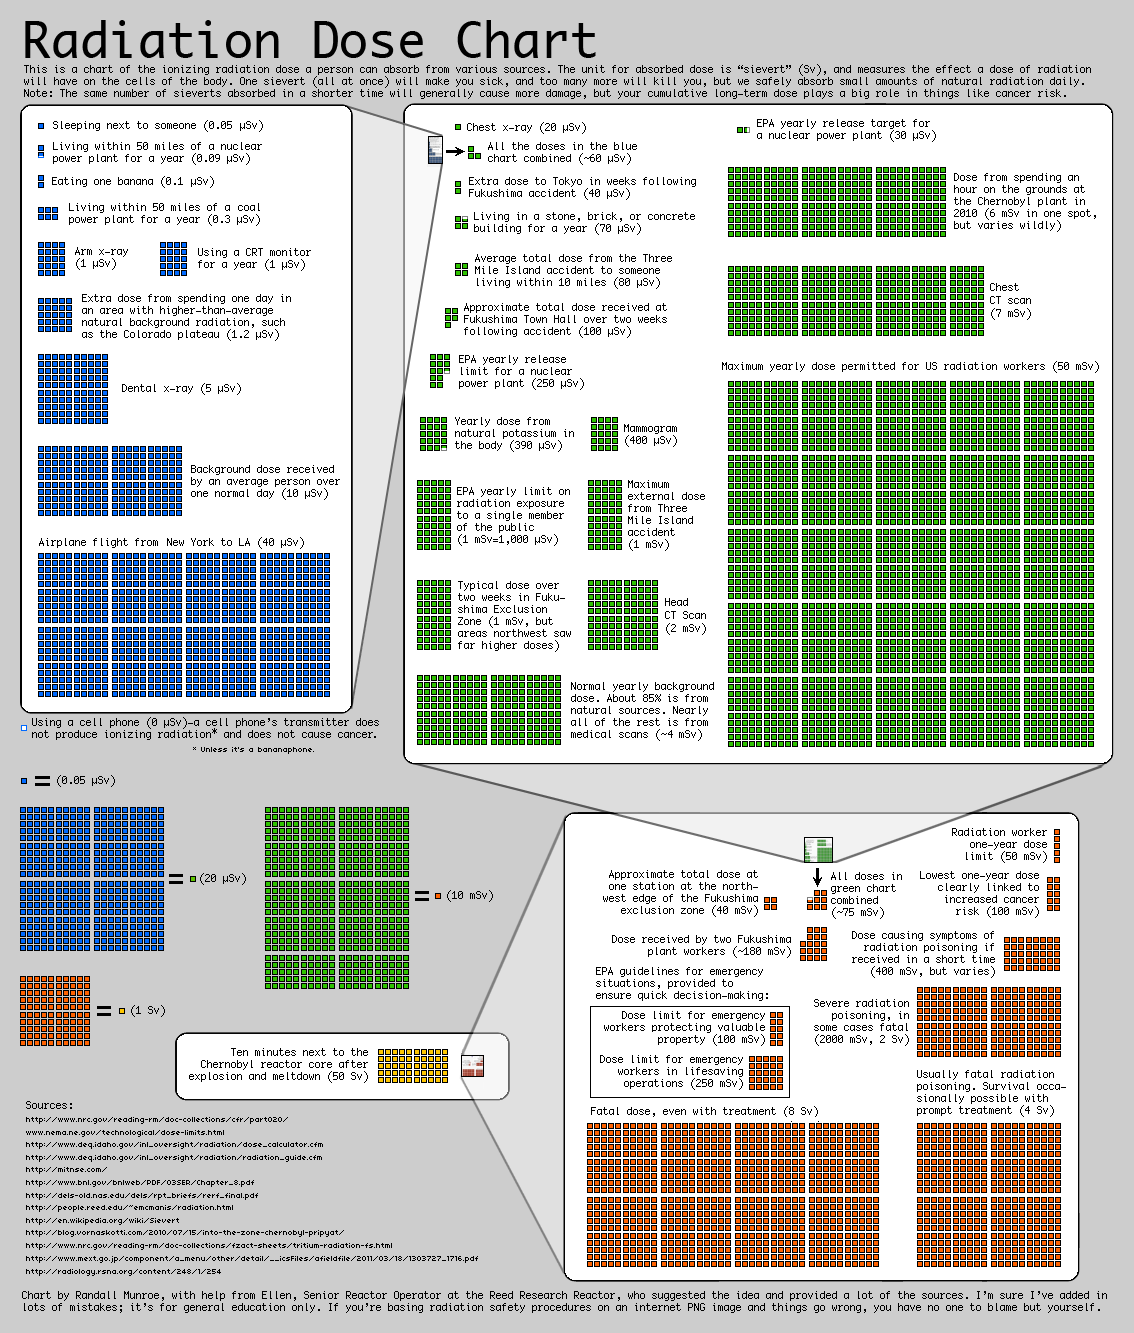
\includegraphics[width=\textwidth]{radioactivity-1/radiation-xkcd}
	\caption{A chart of ionizing radiation dose from various sources. Source: \url{https://xkcd.com/radiation/}}\label{rad1:doses}
\end{figure}

\subsection{Theory of counting statistics}

If you've ever worked in a not-too-busy retail environment, you’ve probably had the
experience of realizing (perhaps) that random and uniform are two quite different things.
You no doubt have sat waiting for customers, with nobody around for long stretches of
time, and then, as though they'd coordinated in advance, a half dozen people all show up
within a few minutes of each other. Each customer is indeed independent (no, they didn't
have a Twitter call to organize a flashmob!\footnote{Yes, popular interest in flash mobs peaked in 2011. Bear with us here.}) yet their arrival times clearly appear clustered. They are, in fact. But randomly. Uniform – one customer each minute – is quite dramatically different than a random procedure that yields one customer per minute on average. Retail customers (to a great extent), and elementary particles, act randomly, not uniformly.

Each atom in a radioactive sample has, per unit time, some probability of undergoing
radioactive decay. That probability is independent of all the other atoms in the sample.
Each atom decays, or not, based on its own probability and no other. The ensemble of
particle decay counts that one would measure in the sample (using a Geiger counter as we will
do, for example) is described by the something called the Poisson distribution, which
gives, in this instance, the probability of a integer number of events occurring in a fixed
interval of time, given an average rate. For large count rates, like we have here, the
Poisson distribution is indistinguishable from the normal distribution (that is, a simple
Gaussian function).

Specifically, for a process that produces an average $\bar{N}$ counts in a certain time duration (in the case of large $N$), the expected measurement of that count for that time duration is a
random draw from a normal distribution with mean $\bar{N}$ and a standard deviation of
$\sqrt{N}$.

\begin{framed}
	\textbf{The Apparatus.}
	
	The energetic particles produced in radioactive decay reactions can be detected by a
	device called a Geiger counter. This consists of a tube filled with inert gas with a wire
	running through it. A high voltage is applied between the wire and the tube. When a high-
	energy particle enters the tube, it can ionize the gas. The freed electrons produce a brief
	pulse of current at the output of the device. The pulses can then be counted.
	
	The counter itself is controlled using buttons on the front panel. \texttt{COUNT} begins the count
	and starts the timer, \texttt{STOP} pauses the count and timer, and \texttt{RESET} sets the count and
	timer to zero. Use the dial on the counter to change the display between the count and the
	elapsed time. When you first turn on the Geiger counter you need to set the voltage to
	$1000\:$V --- the TA will demonstrate how. \textbf{Caution:} Do not turn off the voltage during the
	experiment; use the \texttt{STOP} button to stop the count. \textbf{Do not touch the window on the
		bottom of the tube, as it breaks extremely easily.}
\end{framed}

\section{Procedure}

Your task is to measure the half-life of $^{108}$Ag. We will use the Geiger tube to count
decays. That is, we will count the $\beta$ particles --- the gamma rays make only a small
contribution to the counts in this instance. You should attempt to carry out the counting
fairly quickly after the silver foil is removed from the howitzer as the decay time is quite
short.

\begin{steps}
	\item Before the neutron irradiation begins you will want to record the background rate. Press
\texttt{STOP} and \texttt{RESET} on the counter to set the display to zero.

	\item Next, press \texttt{COUNT} with no
sample below the Geiger tube and collect the total number of background counts, $N_\textrm{bkg}$ ,
that accumulate in approximately 5 minutes. Once 5 minutes has elapsed press \texttt{STOP} to
end the count.

	\item Turn the dial to \texttt{TIME} and record a precise measurement of the elapsed
time, $t$, in seconds. The background rate $R_\textrm{bkg}$ is found with
\begin{equation}
R_\textrm{bkg} = N_\textrm{bkg} /t
\end{equation}
with an uncertainty given by Poisson statistics. \textbf{Report both the background rate and uncertainty in your lab report.}

	\item While the samples are being irradiated, set up your measurement apparatus.

	\item Once the samples are ready, quickly place a silver foil sample in the tray below the Geiger tube. Using a stopwatch and the counter, record the number of counts and the time at 30 second intervals for about 10 minutes, continuously.%
%Unlike last week's lab with the same apparatus, you will be recording data continuously, and so
You will need to use the watch to record times rather
than timer built into the Geiger counter. \textbf{Record your data.} \textit{You may want to take a video of the stopwatch and counter to get more precise readings of the 30-second intervals.}
\end{steps}


\section{Calculations}

The experimental data will be used to determine a half-life (or half-lives). We know that
the decay rate ($R=\Delta N / \Delta t$) of a radioactive nuclide is proportional to the number of nuclei present. The proportionality constant is called the decay constant $\lambda$, and the equation that describes what was just discussed is
\begin{equation}
 R = \lambda N \,,
\end{equation}
where $N$ is the background-subtracted counts. Using integral calculus and the above equation, we find
\begin{equation}
 \frac{N}{N_0} = e^{-\lambda t} \,,
\end{equation}
where $N_0$ is the number of nuclei at the initial time $t=0$. The half life $T_{1/2}$ is defined by
the time it takes for $N = N_0 /2$ and is related to the decay constant by $T_{1/2} = \ln(2)/ \lambda$, where
$\ln()$ is the natural logarithm function, and so $\ln(2) \approx 0.693$.

We can now write the radioactive decay equation as
\begin{equation}
 R = \lambda N_0 e^{-t \ln(2) / T_{1/2}} \,.
\end{equation}
Taking the logarithm of both sides and substituting for $N$ gives
\begin{equation}
 \ln(R) = - \left(\frac{\ln(2)}{T_{1/2}} \right) t + \mathrm{const} \,.
\end{equation}
Your TA will help you to understand the details of this derivation.

\begin{steps}
	\item Make a plot showing $\ln(R)$ on the vertical axis and elapsed time, $t$, along the horizontal axis. Don’t forget to subtract the background where appropriate.

	\item Calculate the slope and use this value to solve for the half life using the above equations. \textbf{Report this value along with a table of your decay rate data and the plot described above.}
\end{steps}

\section{Questions (these should be included in your lab report)}

\begin{steps}
	\item Look up the half-lives of the various nuclides of silver. What is the published
	half-life of the nuclide you’re observing? How does this compare with your
	calculated result? Calculate the percent difference in your result.
	
	\item For the silver foil, how long would it take before you would expect to detect only
	one count per second, background corrected?
	
	\item The detector only measures particles that travel up into the detector. The majority
	of particles traveling in the other directions escape detection. Will this short-
	coming affect the measured half-life? If so, how? If not, why not?
	
	\item Describe one thing you could change in this experiment that could lead to a more
	accurate measurement of the half-life of the silver isotope.
	
	\item The particular irradiated silver sample you used contained some unknown
	percentage of the unstable silver isotope, and was irradiated at some unmeasured
	time before you began your experiment. Does this matter to your results? Explain.
	
\end{steps}

\section{Report checklist and grading}

Each item below is worth 10 points, and there is an additional 10 points for attendance and participation.

\begin{enumerate}
	\item Background rate and uncertainty (Step 3)
	
	\item Plot of $\ln(R)$ vs.\ $t$ with the trendline and equation listed. (Step 6)
	
	\item Calculation of slope of above plot and work of solving for the half-life, with the final half-life determination. (Step 7)
	
	\item Answers to questions in Steps 8--9.
	
	\item Answers to questions in Steps 10--12.
\end{enumerate}
%\chapter{Using light waves to measure small distance changes (Michelson interferometer)}

\section{Introduction}

With the basic properties of waves and wave interference established (via the ripple tank) and the same behavior
demonstrated in light (via the laser-based modern version of Young's double slit experiment) we are now finally ready to
look at a Michelson interferometer. This technology is the basis of the LIGO experiment. You may want to refer back to
the introduction of Lab~\ref{cha:ripple-tank} to remind yourself of some details. LIGO itself is a large experiment that has
been constructed over several decades of work and technology development, and so is many orders of magnitude more
precise and sensitive than what we can do in an hour on a lab bench. Nevertheless, the basic principles are the same.

%\section{Learning Goals}

\section{Team roles}

\begin{steps}
	\item \textbf{Decide on roles} for each group member.
\end{steps}

The available roles are:

\begin{itemize}
	\item Facilitator: ensures time and group focus are efficiently used
	\item Scribe: ensures work is recorded
	\item Technician: oversees apparatus assembly, usage
	\item Skeptic: ensures group is questioning itself
\end{itemize}

These roles can rotate each lab, and you will report at the end of the lab report on how it went for each role. If you have fewer than 4 people in your group, then some members will be holding more than one role. For example, you could have the skeptic double with another role. Consider taking on a role you are less comfortable with, to gain experience and more comfort in that role.

Additionally, if you are finding the lab roles more restrictive than helpful, you can decide to co-hold some or all roles, or think of them more like functions that every team needs to carry out, and then reflecting on how the team executed each function.

\section{Add members to Canvas lab report assignment group}

\begin{steps}
	\item On Canvas, navigate to the People section, then to the ``Lab 3 Groups'' tab. Find a group that is not yet used, and have each person in your group add themselves to that same lab group.
\end{steps}

This enables group grading of your lab report. Only one person will submit the group report, and all members of the group will receive the grade and have access to view the graded assignment.

\section{Observation experiment: demonstration of the interferometer}

\subsection{Goal}

Observe the flow of light in the Michelson interferometer simulation.

\subsection{Available equipment}

\begin{itemize}
	\item A virtual Michelson interferometer found at \url{https://www.geogebra.org/m/msfpudej}
	\begin{itemize}
		\item Note: in the sim, do not zoom in and out by scrolling --- when this happens, the coordinate system appears to shrink and expand, leading to the mirrors seeming to move in space.
	\end{itemize}
\end{itemize}

\subsection{Rubrics to be assessed for this section}

None.

\section{Steps}

\begin{steps}
	\item Load the virtual apparatus at the address listed in the available equipment section.
	
	\item Click the refresh button in the simulation, to the right of the Zeit slider. This fixes a bug where the green wave does not fully display.

	\item Slide Zeit (German for "time") to the left to equal 0. Uncheck "Weg Spiegel 1" (wave path 1)
\end{steps}

This is the Michelson interferometer, invented by Albert Michelson, a physicist whose family immigrated to the USA from Poland when he was 2 years old. He grew up in mining camps in California and Nevada and went on to found the physics department here at UChicago. Let's walk through the operation of the interferometer step by step. A schematic of the setup with parts labeled is found in Figure\ \ref{mir:fig:setup}.

\begin{figure}
	\centering
	\includegraphics[width=\textwidth]{michelson-interferometer-remote/michelson-setup-geogebra}
	\caption{Diagram of the Michelson interferometer simulation with parts labeled.}\label{mir:fig:setup}
\end{figure}

\begin{steps}
	\item Select "Animation" and watch as the wave leaves the laser source and select it again to pause as the wave encounters the beam splitter.
\end{steps}

The beam splitter is a device that reflects some of the beam and transmits the rest. This one is a 50/50 beam splitter, so it splits the beam into equal parts.

\begin{steps}
	\item Select "Animation" again to watch the reflected part of the beam travel until it reaches the output/viewing screen. You'll watch the transmitted part of the beam at a later step. For now it is not displayed. \textit{If the reflected beam does not appear, refresh the animation using the circular arrow button to the right of the Zeit slider.}
\end{steps}

This reflected beam travels to the stationary mirror a distance $d_2$, reflects from that mirror, travels directly through the beam splitter on the way back, and exits the device to be seen on the viewing screen. (we ignore the part that is reflected when it strikes the beam splitter on the way back). The arrow that appears at the output represents the phase of the wave that is passing that point. For example, when the wave is cresting, the arrow points up, and when the wave is at a trough, the arrow points down.

\begin{steps}
	\item Move Zeit back to zero. Check the box for Weg Spiegel 1 and uncheck Weg Spiegel 2. Watch the animation again to follow the path of the beam that is initially transmitted through the beam splitter.
\end{steps}

This beam strikes the mirror at $d_1$, which is movable using the slider on the left or by typing in the desired distance. The typing field accepts numbers with precision up to 4 decimal places.

\begin{steps}
	\item Move Zeit back to zero, check both boxes, and watch the beams overlap with each other at the output.
\end{steps}

In this way the original beam of light splits, and portions of the resulting beams are brought back together to interfere with each other. The black arrow represents the sum of the two waves. The direction is the phase and the length is proportional to the amplitude of the resulting wave.

\section{Testing experiment: testing the theory of wave interference}

\subsection{Goal}

Test if the theory of wave interference and path length difference predicts the correct behavior in the situation of the Michelson interferometer. This theory states that for two different sources of waves that are of the same, single wavelength, and which started out in phase, then constructive interference occurs at a location when the difference in travel distances (path lengths) between the two sources is an integer number of wavelengths. Destructive interference occurs when the path length difference is a half-integer, for example 0.5, 1.5, or 2.5 wavelengths.

\subsection{Available equipment}

\begin{itemize}
	\item A virtual Michelson interferometer as in the previous experiment.
\end{itemize}

\subsection{Rubrics to be assessed for this section}

\begin{itemize}
	\item \textbf{C4:} Is able to make a reasonable prediction based on a hypothesis
	\item \textbf{C7:} Is able to decide whether the prediction and the outcome agree/disagree
	\item \textbf{F1:} Is able to communicate the details of an experimental procedure clearly and completely
	\item \textbf{F2:} Is able to communicate the point of the experiment clearly and completely
\end{itemize}
See Appendix~\ref{cha:rubrics} for details.

\subsection{Suggestions for your experiment}

\begin{itemize}
	\item Ensure that all group members are familiar with how path length difference results in constructive and destructive interference.
	
	\item Examine the geometry of the setup to determine the path length of the beam that travels through each arm of the interferometer.
	
	\item Develop a specific prediction of what setting combinations of wavelength and mirror distance will result in different observable interference effects.
	
	\item Note that in the simulation, you can type in a mirror distance $d_1$ with a precision of 4 decimal places. Press enter after typing it in to save it and have the result displayed.
\end{itemize}

\subsection{Items to include in your report}

Relevant rubric rows from Appendix~\ref{cha:rubrics} are listed in parentheses.

\begin{enumerate}
	\item Clear statement of the hypothesis you are testing (C1, not assessed) [2 pts]
	\item Prediction that follows from the hypothesis, along with justification (C4) [2 pts]
	\item Description of experimental procedure to produce outcome (F1) [2 pts]
	\item Determination of how much the prediction agrees with the outcome (C7) [2 pts]
	\item A discussion of the findings of the experiment and why it's helpful (for you and/or for science) (F2) [2 pts]
\end{enumerate}

\section{Application experiment: measuring length changes with the interferometer}

\subsection{Goal}

The Michelson interferometer is used for LIGO since gravitational waves create very small vibrations in spacetime as they pass. These vibrations literally alter the distance between the beam splitter and mirror along one axis. This MI simulates this with a movable mirror. Using this virtual MI, \textbf{develop a procedure} to determine the change in mirror distance $d_1$ if given the image of the black arrow as displayed on the screen (the arrow's length is proportional to the brightness at that location and moment). \textbf{Demonstrate this procedure} with an example initial and final mirror position.

\textbf{Determine how small} a change in the mirror distance you can measure using your procedure (the \textit{resolution} of the instrument. \textbf{Identify methods} to improve this resolution. 

\subsection{Available equipment}

\begin{itemize}
	\item A virtual Michelson interferometer as in the previous experiment.
\end{itemize}

\subsection{Rubrics to be assessed for this section}

\begin{itemize}
	\item \textbf{D2:} Is able to design a reliable experiment that solves the problem
	\item \textbf{G2:} Is able to evaluate specifically how identified experimental uncertainties affect the data
	\item \textbf{G3:} Is able to describe how to minimize experimental uncertainty and actually do it
	\item \textbf{F1:} Is able to communicate the details of an experimental procedure clearly and completely
	\item \textbf{F2:} Is able to communicate the point of the experiment clearly and completely
\end{itemize}

See Appendix~\ref{cha:rubrics} for details.

\subsection{Suggestions for your experiment}

\begin{itemize}
	\item Remember that the laser wavelength $\lambda$ and the mirror distances are given in micrometers ($\mu$m). This makes it an infrared laser.
	
	\item Decide how you will measure the black arrow's length. This can many methods, for example holding up a ruler to the screen or taking a screenshot and measuring the pixel length in an image analysis program like ImageJ.
	
	\item Note that in the simulation, you can type in a mirror distance $d_1$ with a precision of 4 decimal places. Press enter after typing it in to save it and have the result displayed.
\end{itemize}

\subsection{Items to include in your report}

Relevant rubric rows from Appendix~\ref{cha:rubrics} are listed in parentheses.

\begin{enumerate}
	\item Description of procedure to use image of black arrow to determine the change in mirror distance $d_1$ (D2, F1) [2 pts]
	\item Demonstration of this procedure [2 pts]
	\item Determination of measurement resolution (G2) [2 pts]
	\item Identification of ways to improve this resolution (G3) [2 pts]
	\item A discussion of the findings of the experiment and why it's helpful (for you and/or for science) (F2) [2 pts]
\end{enumerate}

\section{Group functioning}

\begin{steps}
	\item A 100--200 word reflection on group dynamics. Address the following topics: who did what in the lab, how did you work together, how group roles functioned, what successes and challenges in group functioning did you have, and what do you want to continue doing or do differently?
\end{steps}

\section{Individual homework}

\begin{enumerate}
	\item If you were to add a mirror between the beam splitter and the movable mirror, such that the light struck the movable mirror, then our new mirror, then back to the movable mirror, then back to the beam splitter, how would this change the resolution of your measuring device from the application experiment, if at all?
	
	\item Given the resolution of your instrument that you found in the application experiment, what are examples of objects at that length scale that you would be able to use this to measure with 1\% accuracy? You can use this website as a starting point: \url{https://htwins.net/scale2/}
\end{enumerate}
%\chapter{Behavior of gravity waves in water (the ripple tank)}\label{cha:ripple-tank}

%TODO include theoretical limit considerations in curve fitting
%TODO for experiment 3, split setup into discrete Steps. Bold instructions to document things.
%TODO add falstad ripple tank link

\section{Introduction}

The Michelson interferometer, named after University of Chicago professor Albert A. Michelson (Nobel prize in Physics 1907), is an extremely sensitive instrument capable of measuring incredibly tiny displacements.
A modern version of the Michelson interferometer has been developed by The Laser Interferometer Gravitational-Wave Observatory (LIGO) experiment to detect changes in distance of $10^{-19}\:$m (much less than the size of the nucleus of an atom!).
This displacement is sensed between mirrors separated by 4 km (see Figure~\ref{rt:fig:ligo-aerial}). There are two sites for LIGO --- one in Hanford, WA and the other in Livingston, LA.
The LIGO interferometer has recently detected gravitational waves for the first time (September 15, 2015); the first announced gravitational wave detection fits, with remarkable precision, the expected signal from the merging of two black holes, 29 and 36 solar masses, located 410 Mpc away.
The reported signal and the comparison to the fitted model are shown in Figure~\ref{rt:fig:ligo-signals}.

\begin{figure}
	\includegraphics[width=\textwidth]{ripple-tank/ligo-aerial.png}
	\caption{An aerial view of the two LIGO sites.}\label{rt:fig:ligo-aerial}
\end{figure}

\begin{figure}
	\centering
	\includegraphics[width=0.7\textwidth]{ripple-tank/ligo-signals.png}
	\caption{The left panels show the LIGO signal at the Hanford site (top) and the best-fit model
		(middle) and the residual of the model minus the data (bottom). The residuals are consistent
		with noise. The right panels show the same for the Livingston site, with the Hanford signal
		plotted in red in the top panel to demonstrate the similarity of the two measurements (as
		expected in the event of a true gravitational wave signal). This first LIGO detection of a
		gravitational wave event marks a significant transformation in our collective ability to
		measure and understand black holes, and since that first detection, more black hole merger
		events have been detected and reported.}\label{rt:fig:ligo-signals}
\end{figure}

The working principle of the Michelson interferometer is the interference of light.
In this lab, you will first explore the concepts of interference with waves produced in water, in a device known as a ripple tank.
In particular, in this first portion of the lab you will experimentally verify a relationship between wave frequency and wavelength, and then demonstrate constructive and destructive wave interference.
You will then extend that understanding of interference to a wave geometry more appropriate to the second portion of the lab.
The final measurement with the ripple tank will allow you to show that plane waves propagating through a slit behave as though the slit were a new source of waves, propagating radially (i.e.\ in a circular pattern).

Next week, you will measure interference phenomena with light, with a modern version of the famous double-slit experiment performed by Thomas Young in 1801.
You will show that the interference properties of waves established in the first section of the lab apply to light as well, thus experimentally demonstrating that light behaves in a wavelike manner.

Having established the wavelike nature of light, you will then finally use a table-top Michelson interferometer to measure changes in distances smaller than a human hair (not quite LIGO sensitivity, but still pretty impressive!).

\section{Learning Goals}

\begin{itemize}
	\item Learn how to conduct an observational experiment, including collecting data and analyzing the data to find and describe a pattern quantitatively.
	
	\item Discover the relationship between frequency and wavelength of waves.
	
	\item Learn how to conduct a testing experiment, including identifying a hypothesis, designing an experiment, making a prediction, and comparing it to an experimental outcome.
	
	\item Gain familiarity with wave interference.
\end{itemize}

\section{Initial planning for your project and presentation.}

Later in the course, you will write a project paper and make a presentation in lab section  on the same topic.  Project topic choices and presentation dates must be arranged with, and approved by your TA. Your choice of topic must be made in consultation with TAs and other students, so that no more than one person in any section will present on any given topic. A listing 
of ``pre-approved'' project topics is provided on Canvas. Other topics can also be accepted, with prior approval.

During the first week in lab section, \textbf{discuss the options with your TA and other students}.  By the end of your  second  lab section meeting, mutually agree on plans for your course project topic and presentation date.

\section{Group formation}

\begin{steps}
	\item Once you have a group, meet with each other and decide a) what tools you will use to communicate and collaborate, b) when you will meet, c) what you will do when you need to change an agreement, and d) what you will do when a member has a concern about how the group is functioning. \textbf{Record your agreements in your lab report.} %This part counts as data collection and analysis, so it can be identical in each member's report.}
\end{steps}

\subsection{Team roles}

\begin{steps}
\item \textbf{Decide on roles} for each group member.
\end{steps}

The available roles are:

\begin{itemize}
\item Facilitator: ensures time and group focus are efficiently used
\item Scribe: ensures work is recorded
\item Technician: oversees apparatus assembly, usage
\item Skeptic: ensures group is questioning itself
\end{itemize}

These roles can rotate each lab, and you will report at the end of the lab report on how it went for each role. If you have fewer than 4 people in your group, then some members will be holding more than one role. For example, you could have the skeptic double with another role. Consider taking on a role you are less comfortable with, to gain experience and more comfort in that role.

Additionally, if you are finding the lab roles more restrictive than helpful, you can decide to co-hold some or all roles, or think of them more like functions that every team needs to carry out, and then reflecting on how the team executed each function.

\subsection{Add members to Canvas lab report assignment group}

\begin{steps}
\item On Canvas, navigate to the People section, then to the ``L1 Ripple'' tab. Find a group that is not yet used, and have each person in your group add themselves to that same lab group.
\end{steps}

This enables group grading of your lab report. Only one person will submit the group report, and all members of the group will receive the grade and have access to view the graded assignment.

\section{The Scientific Cycle\protect\footnote{adapted from \cite{etkina_college_2014}}}

One way of describing science is the process of incrementally improving a shared model of how our universe works. In different fields of science, different methods and cycles are used, so there is no ``One True Scientific Method.'' One can still create a model for the process of science, and we describe here one such cycle (the hypothetico-deductive cycle), summarized in Figure~\ref{me:fig:isle}.

In this cycle, there are three types of experiments, each one representing a different stage of the scientific effort. One stage, often started when encountering a novel phenomenon, is the \textbf{observational experiment}. This is an experiment that consists of deciding what to observe and how to observe it, collecting data, finding a pattern, and brainstorming possible explanations for what is observed (also called ``hypotheses'').

Once one has some trial explanations, one can test one or more of those with a \textbf{testing experiment}. Here, one designs a new experimental procedure and uses each hypothesis to predict what will happen. Then the prediction is compared to the procedure's outcome. If they are different, then the hypothesis is judged to be not a helpful explanation for that phenomenon. If they are the same, then it is still helpful. Throughout this stage, one may make various assumptions that would need to be validated, as they can effect the prediction or outcome.

Once a hypothesis has been tested enough for people to find it useful, then it can be applied to solve practical problems, or to determine properties of particular situations, in an ``application experiment.''

\begin{figure}
	\centering
	\includegraphics[width=0.7\textwidth]{ripple-tank/islegraphic.png}
	\caption{A model of the process some scientists go through to create knowledge.\cite{etkina_millikan_2015}}\label{me:fig:isle}
\end{figure}

\section{Experiment 1: Observation of frequency and wavelength}

\textbf{Goal:} Observe gravity waves in a ripple tank and determine a mathematical relationship between frequency and wavelength.

\textbf{Available equipment:} ripple tank with strobe light and ripple generator, plane wave attachment, 2 dippers (narrow plastic rods), 1 short wall, 1 medium wall, 2 long walls for ripple tank, flashlights or desk lamps, digital camera (e.g.\ your smartphone), computer with ImageJ installed (can be your device), object of known size to be submerged. You can also use a virtual ripple tank found at \url{www.falstad.com/ripple}.

\begin{framed}
	\textbf{Caution: Flickering Lights!} You will be using a stroboscopic light in this lab. Such light is known to trigger reactions in some individuals (e.g. photosensitive epilepsy).
	If you are worried that you may be sensitive to strobe light, speak to the TA and skip attending this part of the lab.
	In any case, avoid staring directly at the light.
\end{framed}

\begin{framed}
	\textbf{Self-assessment:} To help you improve your scientific abilities, we provide you with self-assessment rubrics.
	A rubric is a scoring system.
	Self-assessment is determining how well you performed a particular task.
	So, these self-assessment rubrics are designed to help you evaluate your performance while you are designing and performing your experiment.
	
	The complete set of rubrics is available in Appendix~\ref{cha:rubrics}.
	In each lab, your report will be assessed using Rubric F, found in Table~\ref{rubric:f}, as well as 5 additional rubric rows listed in that lab.
	Each week, read through these and use them to evaluate your work as you design and perform the experiment.
	Your instructor will use the same rubrics to determine part of your grade for the lab.
\end{framed}	

\textbf{Rubrics to focus on during this experiment:} B7, B8, F1, F2. See Appendix~\ref{cha:rubrics} for details.

\subsection{The ripple tank and generator}

In this section you will explore interference phenomena using a ripple tank. The tank --- 42.5 cm x 42.5 cm and 2.5
cm deep --- is filled with water, and is equipped with a ripple generator. The generator uses voice coil actuators to
produce the precise and quiet up-and-down motion of the rippler arms. Waves are generated in the tank by the moving
dippers that touch the surface of the water. The generator also controls a light source that produces a bright, clear
image of the wave patterns in the ripple tank. The light can be used as a steady source or as a strobe to ‘freeze’ the
motion of the wave patterns (in this case the flashing light and the generator are driven with the same frequency). The
ripple generator frequency ranges from 1.0 to 50 Hz adjustable in 0.1 Hz increments. You will work with frequencies in
the range 16--32 Hz. A mirror placed below the tank and working in conjunction with a projection screen provide a
magnified image of the wave patterns in the water; you will record patterns seen on this screen by photographing them
with a digital camera. The ripple generator terminates in a bar with numerous clips in which you can place various
``dippers''.

\subsection{Suggestions for your experiment}

\begin{enumerate}

	\item Ensure that every group member knows what the terms frequency and wavelength mean, in relation to waves. Use whatever means at your disposal to do this.
	
	\item This is an ``observational experiment.'' Review Rubric B (Table~\ref{rubric:b}) and discuss any unclear expectations with your group and the instructor. Note that your lab report will be graded, in part, on demonstration of Abilities B7 and B8.
	
	\item Ensure that one of the ripple tank's ripple generator is set up with 1 dipper fixed in the center clip of the bar that extends from the box, and that the height of the generator is such that the dipper just touches the top of the water. You can make coarse adjustments by moving the generator along the support rod, and fine adjustments with the two red knobs on it.
	
	\item Brainstorm different methods you could use to determine the relationship between wavelength and frequency. Feel free to play with the ripple tank as you do so, seeing what the frequency and amplitude knobs do. Notice that for different frequencies, different amplitudes produce the clearest image. Here are some things to consider:
	\begin{itemize}
		\item Which variable will you control (and thus will be the independent variable) and which will you measure?
		
		\item What is the range of the independent variable that you will use? How many different settings will you choose?
		
		\item You will need to use several settings of the independent variable, and then plot the data in a graph, decide on what pattern you see, and give some justification for that pattern. You can use words like ``proportional'', ``linear'', ``parabolic'', ``exponential'', ``logarithmic'', and so on, if they fit. Ensure you use the mathematical definition of these.
		
		\item How will you measure the wavelength?
		\begin{itemize}
			\item Is it a more precise measurement if you measure several of them at once and divide to get a single wavelength?
			
			\item The reflected image might magnify the ripple tank, so it can be helpful to place an object of known size in the tank, like a coin, so you can determine the correct scaling.
		\end{itemize}
		
		One way to take careful measurements of the wavelength is to take a picture of the projected tank, then use a program like ImageJ to measure the lengths you need. If you do so, one way to keep track of what settings go with what image is to mark a card with the settings and place it in view of the camera. See the section below on measuring lengths with ImageJ.
	\end{itemize}

	\item Decide on your measurement and analysis method and discuss it with an instructor before you begin. They will help increase the chances that your method will lead to successful results, or at least that the unhelpful path that you choose will take a short enough amount of time for you to change it when you discover it does not work. We want you to have productive failure that you have time to learn from.
	
	\item Perform your experiment. Your lab report for this experiment should include:
	\begin{itemize}
		\item A labeled sketch or photo of the setup, and a description of the experimental procedure (see Rubric F1) [2 points].
		
		\item A plot of wavelength vs. frequency (with the independent variable on the horizontal axis) [1.5 points]
		
		\item A description of the pattern found. This can be done with a line (straight or curved) showing the pattern you see (either drawn manually or using the curve fitting function of the plotting program, e.g.\ LibreOffice Calc or Microsoft Excel) and with words describing what you found. (B7) [1.5]
		
		\item An equation to represent the pattern. This can be taken from a curve fit or found by hand. Make sure there is some discussion of how well the equation agrees with the data, but you don't need to be very precise about it. (B8) [1.5]
		
		\item A discussion of the findings of the experiment and why it's helpful (for you and/or for science) (F2) [2]
	\end{itemize}

\end{enumerate}

\subsection{Measuring lengths using ImageJ}

ImageJ (\url{http://imagej.nih.gov/ij/download.html}), which is installed on the lab computers, is useful for measuring lengths in images. To do so, load your image, then follow these steps to calibrate the ruler --- that is, to tell ImageJ how long something is in the image, so it knows how many pixels correspond to what length).

\begin{enumerate}
	\item Start with an image that has an object in it that you know one of the lengths of (e.g.\ the length of side, or a diameter).
	
	\item Open that image in ImageJ.
	
	\item Select the icon with the straight line on it, and click and drag along the known length.
	
	\item From the drop-down menu, select ``Analyze'' $>$ ``Set Scale...''.
	
	\item Set ``Known distance'' to the value of the known length.
	
	\item Set ``Unit of length'' to the unit you are using, for example ``mm'' for millimeters.
	
	\item Record the pixel scale given at the bottom of the box for future use.
	
	\item Now when you use the straight line tool, it will give the length in physical units in ImageJ's toolbar.
\end{enumerate}

\section{Experiment 2: Testing the conditions for constructive interference}

\textbf{Goal:} A student in another physics class is trying to remember the equation for constructive interference between waves. Their best guess is that constructive interference between two waves occurs at positions where the distance from each source differs by a half-integer number of wavelengths, or
\begin{equation}
 \Delta d = (m+\frac{1}{2})\lambda \,,
\end{equation}
where $\Delta d$ is the ``path length difference'', $\lambda$ is the wavelength, and $m$ is any integer. \textbf{Test the idea represented by the equation to see if the student remembered it accurately.}

\textbf{Available equipment:} Same as in the previous experiment.

\textbf{Setup:} Instead of 1 dipper, use two dippers mounted with 3 empty clips between them on the bar. Ask the TA for assistance in setting this up. Adjust so that the dippers are just resting in the surface of the water. Adjust the frequency and amplitude to get clear, sharp waves.

\textbf{Rubric rows to be assessed in this experiment:} C1, C4, C7, F1, F2. See Appendix~\ref{cha:rubrics} for details.

\subsection{Testing this hypothesis}

In general, one tests a hypothesis by using it to make a prediction about what will happen in a certain experimental procedure. With this hypothesis, it asserts a relationship between path length difference, wavelength, and constructive interference. But there are only certain points on the ripple tank image where it is easy to see constructive interference --- the bright spots at the intersection of waves originating from both sources. For an example, see Figure~\ref{rt:fig:interference-2d}.

\begin{figure}
	\centering
	\includegraphics[width=0.7\textwidth]{ripple-tank/interference-2d.png}
	\caption{Example interference pattern for 2 dippers. The bright spots are circled. For a particular bright spot of constructive interference, the two path lengths PS1 and PS2 are drawn.}\label{rt:fig:interference-2d}
\end{figure}

In this case, it is easier to start by finding those locations, measuring the $\Delta d$, finding the wavelength for the given frequency using the relationship you found in Experiment 1, and solving for $m$. The hypothesis predicts that $m$ should always be an integer. As a result, your experiment becomes this: find out how close the experimentally determined $m$'s are to integers.

Brainstorm your experimental procedure, decide on it, discuss with your TA, then perform the experiment.

Your lab report for this experiment should include:
\begin{itemize}
	\item A clear description of the hypothesis (see Rubric C1) [1.5 points].
	
	\item A labeled sketch or photo of the setup, and a description of the experimental procedure (F1) [2].
	
	\item A clear statement of the prediction that the hypothesis makes for this particular procedure (C4) [1.5].

	\item A table of path lengths, path length differences, and measured $m$ values [1.5].
	
	\item An analysis of how close the measured $m$ values are to the prediction. Use some quantitative measure of this, but don't worry about being precise about uncertainties (C7) [1.5].
	
	\item A judgment about the hypothesis. Is it supported, disproved, or undetermined? (C8, though not assessed this time) [1.5]
	
	\item A discussion of the findings of the experiment and why it's helpful (for you and/or for science) (F2) [2].
\end{itemize}

%In the case of a hypothesis like this one, that includes a proposed equation, there is a useful template for coming up with a prediction:
%\begin{enumerate}
%	\item Note that this hypothesis is asserting that when the equation is true, there is constructive interference (a bright spot). So the goal is to test how true this is.
%	
%	\item Choose which variables you are holding constant, which one is the independent, and which is the dependent variable. In this case, you may not know what $m$ is ahead of time. You could choose it arbitrarily, for example $m=0$ first, and go from there.
%	
%	\item Once you decide on your procedure (which things to measure, how to vary the independent variable), you can use the equation to solve for the dependent variable, which becomes the prediction (Rubric C4).
%	
%	\item The set of dependent variables (for each chosen independent variable) becomes the prediction of the hypothesis that you will use to compare to experimental outcome (C7).
%\end{enumerate}
%
%\subsection{Suggestions for your experiment}
%
%\begin{itemize}
%	\item Note that constructive interference happens where there are bright spots in the projected image at the intersection of waves coming from both sources.
%	
%	\item There is an entire line of points that have the same path length difference from each source, so for each choice of $m$, there can be many 
%\end{itemize}

\section{Experiment 3: Observing plane waves encountering narrow gaps}

This experiment does not clearly follow the model of the scientific cycle, but is closest to an observational experiment. In next week's lab, you will investigate the properties of light traveling through small slits. Ripples in water are more obviously waves, so it is helpful to observe what happens here first.

Instead of dippers, remove them and position the bar so that it is resting in the water. This will produce straight line waves, or, in two dimensions, ``plane waves''. This is the same kind of waves we will use next week with light.

Adjust the amplitude and frequency, with the frequency in the range 20--25 Hz, until you see
clear well-defined vertical parallel lines. Now, insert the two large ``walls'' in the tank, parallel to the rippler bar and
perhaps 5cm away; allow a small (few mm) opening between the two wall sections, placed so that opening is vertically
centered in the projected image. Adjust the amplitude upward until you see a clear wave pattern radiating from that
opening. Take a picture. Repeat this with two apertures instead of one; do this by adding a smaller wall between the
two larger sections, with all sections parallel to the rippler bar, and a small gap between each larger wall and the central
smaller portion. Again, take a picture, adjusting amplitude as necessary to get well-defined waves.

The analysis of this will be done as individual homework.

\section{Individual Homework}

These questions are to be answered individually and your answers should be submitted under the Lab 1 Homework assignment on Canvas.

Both questions concern the last two situations recorded in the lab: the case of 2 walls (1 gap or ``aperture'') and the case with 3 walls (2 apertures).

\begin{enumerate}
	\item What wave pattern do you see in the case of a single aperture? What do you see in the case of a double aperture?
	How do these patterns compare to the data you took using dippers on the rippler bar?
	
	\item Is the wavelength of the pattern you observe consistent with the relationship between frequency and wavelength you
	measured with the dippers? Include any measurements and calculations you make in answering this question in your homework response, and be quantitative.
\end{enumerate}

\appendix

\chapter{Analysis of Uncertainty}\label{cha:uncertainty}

%todo mark std dev equation and general error propagation formula as optional/advanced - recommend use =STDDEV to compute

A physical quantity consists of a value, unit, and uncertainty.
For example, ``$5 \pm 1\,$m'' means that the writer believes the true value of the quantity to most likely lie within 4 and 6 meters\footnote{The phrase ``most likely'' can mean different things depending on who is writing.
	If a physicist gives the value and does not given a further explanation, we can assume that they mean that the measurements are randomly distributed according to a normal distribution around the value given, with a standard deviation of the uncertainty given.
	So if one were to make the same measurement again, the author believes it has a 68\% chance of falling within the range given.
	Disciplines other than physics may intend the uncertainty to be 2 standard deviations.}.
Without knowing the uncertainty of a value, the quantity is next to useless.
For example, in our daily lives, we use an implied uncertainty.
If I say that we should meet at around 5:00 pm, and I arrive at 5:05 pm, you will probably consider that within the range that you would expect.
Perhaps your implied uncertainty is plus or minus 15 minutes.
On the other hand, if I said that we would meet at 5:07 pm, then if I arrive at 5:10 pm, you might be confused, since the implied uncertainty of that time value is more like 1 minute.

Scientists use the mathematics of probability and statistics, along with some intuition, to be precise and clear when talking about uncertainty, and it is vital to understand and report the uncertainty of quantitative results that we present.

\section{Types of measurement uncertainty}\label{unc:sec:types}

For simplicity, we limit ourselves to the consideration of two types of uncertainty in this lab course, instrumental and random uncertainty.

\subsection{Instrumental uncertainties}

Every measuring instrument has an inherent uncertainty that is determined by the precision	
  of the instrument.
Usually this value is taken as a half of the smallest increment of the instrument's scale. For example, $0.5\:$mm is the precision of a standard metric ruler; $0.5\:$s is the precision of a watch, etc. For electronic digital displays, the equipment's manual often gives the instrument's resolution, which may be larger than that given by the rule above.

Instrumental uncertainties are the easiest ones to estimate, but they are not the only source of the uncertainty in your measured value.
You must be a skillful experimentalist to get rid of all other sources of uncertainty so that all that is left is instrumental uncertainty.

\subsection{Random uncertainties}\label{unc:random}

Very often when you measure the same physical quantity multiple times, you can get different results each time you measure it.
That happens because different uncontrollable factors affect your results randomly.
This type of uncertainty, random uncertainty, can be estimated only by repeating the same measurement several times.
For example if you measure the distance from a cannon to the place where the fired cannonball hits the ground, you could get different distances every time you repeat the same experiment.	
  
For example, say you took three measurements and obtained 55.7, 49.0, 52.5, 42.4, and 60.2 meters. We can quantify the variation in these measurements by finding their standard deviation using a calculator, spreadsheet (like Microsoft Excel, LibreOffice Calc, or Google Sheets), or the formula (assuming the data distributed according to a normal distribution)
\begin{equation}
 \sigma = \sqrt{\sum_{i=1}^{N} \frac{(x_i-\bar{x})^2}{N-1}} \, ,
\end{equation}
where $\{x_1, x_2, \dots, x_N\}$ are the measured values, $\bar{x}$ is the mean of those values, and $N$ is the number of measurements.
For our example, the resulting standard deviation is 6.8 meters. Generally we are interested not in the variation of the measurements themselves, but how uncertain we are of the average of the measurements. The uncertainty of this mean value is given, for a normal distribution, by the so-called ``standard deviation of the mean'', which can be found by dividing the standard deviation by the square root of the number of measurements,
\begin{equation}\label{unc:eq:stdevmean}
\sigma_\textrm{mean} = \frac{\sigma}{\sqrt{N}} \, .
\end{equation}
So, in this example, the uncertainty of the mean is 3.0 meters. We can thus report the length as $52 \pm 3\:$m.

Note that if we take more measurements, the standard deviation of those measurements will not generally change, since the variability of our measurements shouldn't change over time. However, the standard deviation of the mean, and thus the uncertainty, will decrease.

\section{Propagation of uncertainty}\label{unc:sec:prop}

When we use an uncertain quantity in a calculation, the result is also uncertain. To determine by how much, we give some simple rules for basic calculations, and then a more general rule for use with any calculation which requires knowledge of calculus. Note that these rules are strictly valid only for values that are normally distributed, though for the purpose of this course, we will use these formulas regardless of the underlying distributions, unless otherwise stated, for simplicity.

If the measurements are completely independent of each other, then for quantities $a \pm \delta a$ and $b \pm \delta b$, we can use the following formulas:
\begin{equation}\label{unc:add}
\textrm{For } c = a + b \textrm{ (or for subtraction), } \delta c = \sqrt{(\delta a)^2 + (\delta b)^2}
\end{equation}

\begin{equation}\label{unc:mult}
\textrm{For } c = ab \textrm{ (or for division), } \frac{\delta c}{c} = \sqrt{\left(\frac{\delta a}{a}\right)^2 + \left(\frac{\delta b}{b}\right)^2}
\end{equation}

\begin{equation}\label{unc:exp}
\textrm{For } c = a^n,\, \frac{\delta c}{c} = n \frac{\delta a}{a}
\end{equation}

For other calculations, there is a more general formula not discussed here.

%If you are familiar with calculus, you may want to use this general formula for the uncertainty $\delta f$ of a function $f$ of $N$ independent values $x_i$, each with uncertainty $\delta x_i$:
%\begin{equation}\label{unc:general}
%\delta f = \sqrt{ \sum_{i=1}^{N} \left(\frac{\partial f}{\partial x_i} \delta x_i\right)^2 } \, .
%\end{equation}
%Notice that Eqs.\ \ref{unc:add} through \ref{unc:exp} can be derived from Eq.\ \ref{unc:general} for those specific cases.

\subsubsection{What if there is no reported uncertainty?}

Sometimes you'll be calculating with numbers that have no uncertainty given.
In some cases, the number is exact.
For example, the circumference $C$ of a circle is given by $C = 2 \pi r$. Here, the coefficient, $2\pi$, is an exact quantity and you can treat its uncertainty as zero.
If you find a value that you think is uncertain, but the uncertainty is not given, a good rule of thumb is to assume that the uncertainty is half the right-most significant digit.
So if you are given a measured length of $1400\:$m, then you might assume that the uncertainty is $50\:$m.
This is an assumption, however, and should be described as such in your lab report.
For more examples, see Table~\ref{unc:tab:implied}.

\begin{table}
	\begin{center}
		\begin{tabular}{cc}
			\textbf{Expression} & \textbf{Implied uncertainty} \\
			12 & 0.5 \\
			12.0 & 0.05 \\
			120 & 5 \\
			120. & 0.5
		\end{tabular}
		\caption{Expression of numbers and their implied uncertainty.}\label{unc:tab:implied}
	\end{center}
\end{table}

\subsubsection{How many digits to report?}

After even a single calculation, a calculator will often give ten or more digits in an answer.
For example, if I travel $11.3 \pm 0.1\:$km in $350 \pm 10\:$s, then my average speed will be the distance divided by the duration. Entering this into my calculator, I get the resulting value ``\texttt{0.0322857142857143}''.
Perhaps it is obvious that my distance and duration measurements were not precise enough for all of those digits to be useful information.
We can use the propagated uncertainty to decide how many decimals to include.
Using the formulas above, I find that the uncertainty in the speed is given by my calculator as ``\texttt{9.65683578099600e-04}'', where the `\texttt{e}' stands for ``times ten to the''.
I definitely do not know my uncertainty to 14 decimal places.
For reporting uncertainties, it general suffices to use just the 1 or 2 left-most significant digits, unless you have a more sophisticated method of quantifying your uncertainties.
So here, I would round this to 1 significant digit, resulting in an uncertainty of $0.001\:$km/s.
Now I have a guide for how many digits to report in my value.
Any decimal places to the right of the one given in the uncertainty are distinctly unhelpful, so I report my average speed as ``$0.032 \pm 0.001\:$km/s''.
You may also see the equivalent, more succinct notation ``$0.032(1)\:$km/s''.

\section{Comparing two values}\label{unc:sec:comparing}

If we compare two quantities and want to find out how different they are from each other, we can use a measure we call a $t'$ value (pronounced ``tee prime''). This measure is not a standard statistical measure, but it is simple and its meaning is clear for us.

Operationally, for two quantities having the same unit, $a \pm \delta a$ and $b \pm \delta b$, the measure is defined as\footnote{Statistically, if $\delta a$ and $\delta b$ are uncorrelated, random uncertainties, then $t'$ represents how many standard deviations the difference $a - b$ is away from zero.}

\begin{equation}
%t' = \frac{\abs{a-b}}{\sqrt{(\delta a)^2 + (\delta b)^2}}
t' = \frac{\abs{a-b}}{\sqrt{(\delta a)^2 + (\delta b)^2}}
\end{equation}

If $t' \lesssim 1$, then the values are so close to each other that they are indistinguishable. It is either that they represent the same true value, or that the measurement should be improved to reduce the uncertainty.

If $1 \lesssim t' \lesssim 3$, then the result is inconclusive. One should improve the experiment to reduce the uncertainty.

If $t' \gtrsim 3$, then the true values are very probably different from each other.
%
\chapter{Rubrics}\label{cha:rubrics}

%Each lab is graded 50\% on attendance and participation during the lab, and providing evidence in the lab report of completing all steps of the lab, including answering every question. The other 50\% is based on a selection of scientific abilities.

%Each scientific ability rubric row assessed is worth a possible 1 point, with ``Missing'' being 0 points, ``Inadequate'' 1/3 points, ``Needs Improvement'' 2/3 points, and ``Adequate'' 1 point.

The scientific abilities rubrics are found on the following pages.

\begin{landscape}

\begin{longtable}{>{\bfseries}p{0.04\textheight}|>{\bfseries\RaggedRight}p{0.23\textheight}|>{\RaggedRight}p{0.21\textheight}|>{\RaggedRight}p{0.21\textheight}|>{\RaggedRight}p{0.22\textheight}|>{\RaggedRight}p{0.22\textheight}}
	\toprule
	& Scientific Ability
	& Missing & Inadequate & Needs Improvement & Adequate \\ \midrule \endhead
	A11
	& Graph
	& No graph is present.
	& A graph is present but the axes are not labeled. There is no scale on the axes.
	& The graph is present and axes are correctly labeled, but the axes do not correspond to the independent and dependent variables, or the scale is not accurate.
	& The graph has correctly labeled axes, independent variable is along the horizontal axis and the scale is accurate.
	\\
	\bottomrule
	\caption{Rubric A: Ability to represent information in multiple ways}\label{rubric:a}
	\end{longtable}

\begin{longtable}{>{\bfseries}p{0.02\textheight}|>{\bfseries\RaggedRight}p{0.25\textheight}|>{\RaggedRight}p{0.21\textheight}|>{\RaggedRight}p{0.21\textheight}|>{\RaggedRight}p{0.22\textheight}|>{\RaggedRight}p{0.22\textheight}}
		\toprule
		& Scientific Ability
		& Missing & Inadequate & Needs Improvement & Adequate \\ \midrule \endhead
		B1
		& Is able to identify the phenomenon to be investigated
		& No phenomenon is mentioned
		& The description of the phenomenon to be investigated is confusing, or it is not the phenomenon of interest.
		& \midsloppy The description of the phenomenon is vague or incomplete.
		& The phenomenon to be investigated is clearly stated. \\ \midrule
		B2
		& Is able to design a reliable experiment that investigates the phenomenon
		& The experiment does not investigate the phenomenon.
		& The experiment may not yield any interesting patterns.
		& Some important aspects of the phenomenon will not be observable.
		& The experiment might yield interesting patterns relevant to the investigation of the phenomenon. \\ \midrule
		B3
		& Is able to decide what physical quantities are to be measured and identify independent and dependent variables
		& The physical quantities are irrelevant.
		& Only some of physical quantities are relevant.
		& The physical quantities are relevant. However, independent and dependent variables are not identified.
		& The physical quantities are relevant and independent and dependent variables are identified. \\ \midrule
		B4
		& Is able to describe how to use available equipment to make measurements
		& At least one of the chosen measurements cannot be made with the available equipment.
		& All chosen measurements can be made, but no details are given about how it is done.
		& All chosen measurements can be made, but the details of how it is done are vague or incomplete.
		& All chosen measurements can be made and all details of how it is done are clearly provided. \\ \midrule
		B5
		& Is able to describe what is observed without trying to explain, both in words and by means of a picture of the experimental setup
		& No description is mentioned.
		& A description is incomplete. No labeled sketch is present. Or, observations are adjusted to fit expectations.
		& A description is complete, but mixed up with explanations or pattern. Or the sketch is present but is difficult to understand.
		& Clearly describes what happens in the experiments both verbally and with a sketch. Provides other representations when necessary (tables and graphs). \\ \midrule
		B6
		& Is able to identify the shortcomings in an experiment and suggest improvements
		& No attempt is made to identify any shortcomings of the experiment.
		& The shortcomings are described vaguely and no suggestions for improvement are made.
		& Not all aspects of the design are considered in terms of shortcomings or improvements.
		& All major shortcomings of the experiment are identified and reasonable suggestions for improvement are made. \\ \midrule
		B7
		& Is able to identify a pattern in the data
		& No attempt is made to search for a pattern.
		& The pattern described is irrelevant or inconsistent with the data.
		& The pattern has minor errors or omissions. Terms like ``proportional'' used without clarity, e.g.\ is the proportionality linear, quadratic, etc.
		& The pattern represents the relevant trend in the data. When possible, the trend is described in words. \\ \midrule
		B8
		& Is able to represent a pattern mathematically (if applicable)
		& No attempt is made to represent a pattern mathematically.
		& The mathematical expression does not represent the trend.
		& No analysis of how well the expression agrees with the data is included, or some features of the pattern are missing.
		& The expression represents the trend completely and an analysis of how well it agrees with the data is included. \\ \midrule
		B9
		& Is able to devise an explanation for an observed pattern
		& No attempt is made to explain the observed pattern.
		& An explanation is vague, not testable, or contradicts the pattern.
		& An explanation contradicts previous knowledge or the reasoning is flawed.
		& A reasonable explanation is made. It is testable and it explains the observed pattern. \\
		\bottomrule
		\caption{Rubric B: Ability to design and conduct an observational experiment \cite{etkina_scientific_2006}.}\label{rubric:b}
	\end{longtable}

\begin{longtable}{>{\bfseries}p{0.02\textheight}|>{\bfseries\RaggedRight}p{0.25\textheight}|>{\RaggedRight}p{0.21\textheight}|>{\RaggedRight}p{0.21\textheight}|>{\RaggedRight}p{0.22\textheight}|>{\RaggedRight}p{0.22\textheight}}
	\toprule
	& Scientific Ability
	& Missing & Inadequate & Needs Improvement & Adequate \\ \midrule \endhead
	C1
	& Is able to identify the hypothesis to be tested
	& No mention is made of a hypothesis.
	& An attempt is made to identify the hypothesis to be tested but it is described in a confusing manner.
	& The hypothesis to be tested is described but there are minor omissions or vague details.
	& The hypothesis is clearly, specifically, and thoroughly stated.
	\\ \midrule
	C2
	& Is able to design a reliable experiment that tests the hypothesis
	& The experiment does not test the hypothesis.
	& The experiment tests the hypothesis, but due to the nature of the design it is likely the data will lead to an incorrect judgment.
	& The experiment tests the hypothesis, but due to the nature of the design there is a moderate chance the data will lead to an inconclusive judgment.
	& The experiment tests the hypothesis and has a high likelihood of producing data that will lead to a conclusive judgment.
	\\ \midrule
	C4
	& Is able to make a reasonable prediction based on a hypothesis
	& No prediction is made. The experiment is not treated as a testing experiment.
	& A prediction is made, but it is identical to the hypothesis, OR prediction is made based on a source unrelated to the hypothesis being tested, or is completely inconsistent with hypothesis being tested, OR prediction is unrelated to the context of the designed experiment.
	& Prediction follows from hypothesis but is flawed because relevant assumptions are not considered, OR prediction is incomplete or somewhat inconsistent with hypothesis, OR prediction is somewhat inconsistent with the experiment.
	& A prediction is made that follows from hypothesis, is distinct from the hypothesis, accurately describes the expected outcome of the experiment, and incorporates relevant assumptions if needed.
	\\ \midrule
	C5
	& Is able to identify the assumptions made in making the prediction
	& No attempt is made to identify assumptions.
	& An attempt is made to identify assumptions, but the assumptions are irrelevant or are confused with the hypothesis.
	& Relevant assumptions are identified but are not significant for making the prediction.
	& Sufficient assumptions are correctly identified, and are significant for the prediction that is made.
	\\ \midrule
	C6
	& Is able to determine specifically the way in which assumptions might affect the prediction
	& No attempt is made to determine the effects of assumptions.
	& The effects of assumptions are mentioned but are described vaguely.
	& The effects of assumptions are determined, but no attempt is made to validate them.
	& The effects of assumptions are determined and the assumptions are validated.
	\\ \midrule
	C7
	& Is able to decide whether the prediction and the outcome agree/disagree
	& No mention of whether the prediction and outcome agree/disagree.
	& A decision about the agreement/disagreement is made but is not consistent with the results of the experiment.
	& A reasonable decision about the agreement/disagreement is made but experimental uncertainty is not taken into account.
	& A reasonable decision about the agreement/disagreement is made and experimental uncertainty is taken into account.
	\\ \midrule
	C8
	& Is able to make a reasonable judgment about the hypothesis
	& No judgment is made about the hypothesis.
	& A judgment is made but is not consistent with the outcome of the experiment.
	& A judgment is made, is consistent with the outcome of the experiment, but assumptions are not taken into account.
	& A judgment is made, is consistent with the outcome of the experiment, and assumptions are taken into account.
	\\ \bottomrule
	\caption{Rubric C: Ability to design and conduct a testing experiment \cite{etkina_scientific_2006}.}\label{rubric:c}
\end{longtable}

\begin{longtable}{>{\bfseries}p{0.02\textheight}|>{\bfseries\RaggedRight}p{0.25\textheight}|>{\RaggedRight}p{0.21\textheight}|>{\RaggedRight}p{0.21\textheight}|>{\RaggedRight}p{0.22\textheight}|>{\RaggedRight}p{0.22\textheight}}
	\toprule
	& Scientific Ability
	& Missing & Inadequate & Needs Improvement & Adequate \\ \midrule \endhead
	D1
	& Is able to identify the problem to be solved
	& No mention is made of the problem to be solved.
	& An attempt is made to identify the problem to be solved but it is described in a confusing manner.
	& The problem to be solved is described but there are minor omissions or vague details.
	& The problem to be solved is clearly stated.
	\\ \midrule
	D2
	& Is able to design a reliable experiment that solves the problem.
	& The experiment does not solve the problem.
	& The experiment attempts to solve the problem but due to the nature of the design the data will not lead to a reliable solution.
	& The experiment attempts to solve the problem but due to the nature of the design there is a moderate chance the data will not lead to a reliable solution.
	& The experiment solves the problem and has a high likelihood of producing data that will lead to a reliable solution.
	\\ \midrule
	D3
	& Is able to use available equipment to make measurements
	& At least one of the chosen measurements cannot be made with the available equipment.
	& All of the chosen measurements can be made, but no details are given about how it is done.
	& All of the chosen measurements can be made, but the details about how they are done are vague or incomplete.
	& All of the chosen measurements can be made and all details about how they are done are provided and clear.
	\\ \midrule
	D4
	& Is able to make a judgment about the results of the experiment
	& No discussion is presented about the results of the experiment.
	& A judgment is made about the results, but it is not reasonable or coherent.
	& An acceptable judgment is made about the result, but the reasoning is incomplete, OR uncertainties are not taken into account, OR assumptions are not discussed, OR the result is written as a single number.
	& An acceptable judgment is made about the result, with clear reasoning. The effects of assumptions and experimental uncertainties are considered. The result is written as an interval.
	\\ \midrule
	D5
	& Is able to evaluate the results by means of an independent method
	& No attempt is made to evaluate the consistency of the result using an independent method.
	& A second independent method is used to evaluate the results. However there is little or no discussion about the differences in the results due to the two methods.
	& A second independent method is used to evaluate the results. The results of the two methods are compared correctly using experimental uncertainties. But there is little or no discussion of the possible reasons for the differences when the results are different.
	& A second independent method is used to evaluate the results and the evaluation is correctly done with the experimental uncertainties. The discrepancy between the results of the two methods, and possible reasons are discussed.
	\\ \midrule
	D7
	& Is able to choose a productive mathematical procedure for solving the experimental problem
	& Mathematical procedure is either missing, or the equations written down are irrelevant to the design.
	& A mathematical procedure is described, but is incorrect or incomplete, due to which the final answer cannot be calculated. Or units are inconsistent.
	& Correct and complete mathematical procedure is described but an error is made in the calculations. All units are consistent.
	& Mathematical procedure is fully consistent with the design. All quantities are calculated correctly with proper units. Final answer is meaningful.
	\\ \midrule
	D8
	& Is able to identify the assumptions made in using the mathematical procedure
	& No attempt is made to identify any assumptions.
	& An attempt is made to identify assumptions, but the assumptions are irrelevent or incorrect for the situation.
	& Relevant assumptions are identified but are not significant for solving the problem.
	& All relevant assumptions are correctly identified.
	\\ \midrule
	D9
	& Is able to determine specifically the way in which assumptions might affect the results
	& No attempt is made to determine the effects of assumptions.
	& The effects of assumptions are mentioned but are described vaguely.
	& The effects of assumptions are determined, but no attempt is made to validate them.
	& The effects of assumptions are determined and the assumptions are validated.
	\\ \bottomrule
	\caption{Rubric D: Ability to design and conduct an application experiment \cite{etkina_scientific_2006}.}\label{rubric:d}
\end{longtable}

\begin{longtable}{>{\bfseries}p{0.02\textheight}|>{\bfseries\RaggedRight}p{0.25\textheight}|>{\RaggedRight}p{0.21\textheight}|>{\RaggedRight}p{0.21\textheight}|>{\RaggedRight}p{0.22\textheight}|>{\RaggedRight}p{0.22\textheight}}
	\toprule
	& Scientific Ability
	& Missing & Inadequate & Needs Improvement & Adequate \\ \midrule \endhead	
	F1
	& Is able to communicate the details of an experimental procedure clearly and completely
	& Diagrams are missing and/or experimental procedure is missing or extremely vague.
	& Diagrams are present but unclear and/or experimental procedure is present but important details are missing. It takes a lot of effort to comprehend.
	& Diagrams and/or experimental procedure are present and clearly labeled but with minor omissions or vague details. The procedure takes some effort to comprehend.
	& Diagrams and/or experimental procedure are clear and complete. It takes no effort to comprehend.
	\\ \midrule
	F2
	& Is able to communicate the point of the experiment clearly and completely
	& No discussion of the point of the experiment is present.
	& The experiment and findings are discussed but vaguely. There is no reflection on the quality and importance of the findings.
	& The experiment and findings are communicated but the reflection on their importance and quality is not present.
	& The experiment and findings are discussed clearly. There is deep reflection on the quality and importance of the findings.
	\\
	\bottomrule
	\caption{Rubric F: Ability to communicate scientific ideas \cite{etkina_scientific_2006}.}\label{rubric:f}
\end{longtable}

\begin{longtable}{>{\bfseries}p{0.02\textheight}|>{\bfseries\RaggedRight}p{0.25\textheight}|>{\RaggedRight}p{0.21\textheight}|>{\RaggedRight}p{0.21\textheight}|>{\RaggedRight}p{0.22\textheight}|>{\RaggedRight}p{0.22\textheight}}
	\toprule
	& Scientific Ability
	& Missing & Inadequate & Needs Improvement & Adequate \\ \midrule \endhead	
	G1
	& Is able to identify sources of experimental uncertainty
	& No attempt is made to identify experimental uncertainties.
	& An attempt is made to identify experimental uncertainties, but most are missing, described vaguely, or incorrect.
	& Most experimental uncertainties are correctly identified. But there is no distinction between random and instrumental uncertainty.
	& All experimental uncertainties are correctly identified. There is a distinction between instrumental and random uncertainty.
	\\ \midrule
	G2
	& Is able to evaluate specifically how identified experimental uncertainties affect the data
	& No attempt is made to evaluate experimental uncertainties.
	& An attempt is made to evaluate uncertainties, but most are missing, described vaguely, or incorrect. Or the final result does not take uncertainty into account.
	& The final result does take the identified uncertainties into account but is not correctly evaluated. Uncertainty propagation is not used or is used incorrectly.
	& The experimental uncertainty of the final result is correctly evaluated. Uncertainty propagation is used appropriately.
	\\ \midrule
	G3
	& Is able to describe how to minimize experimental uncertainty and actually do it
	& No attempt is made to describe how to minimize experimental uncertainty and no attempt to minimize is present.
	& A description of how to minimize experimental uncertainty is present, but there is no attempt to actually minimize it.
	& An attempt is made to minimize the uncertainty in the final result is made but the method is not very effective.
	& The uncertainty is minimized in an effective way.
	\\ \midrule
	G4
	& Is able to record and represent data in a meaningful way
	& Data are either absent or incomprehensible.
	& Some important data are absent or incomprehensible. They are not organized in tables or the tables are not labeled properly.
	& All important data are present, but recorded in a way that requires some effort to comprehend. The tables are labeled but labels are confusing.
	& All important data are present, organized, and recorded clearly. The tables are labeled and placed in a logical order.
	\\ \midrule
	G5
	& Is able to analyze data appropriately
	& No attempt is made to analyze the data.
	& An attempt is made to analyze the data, but it is either seriously flawed or inappropriate.
	& The analysis is appropriate but it contains errors or omissions.
	& The analysis is appropriate, complete, and correct.
	\\
	\bottomrule
	\caption{Rubric G: Ability to collect and analyze experimental data \cite{etkina_scientific_2006}.}\label{rubric:g}
\end{longtable}

\end{landscape}
\include{report-format-short/report-format-short}
%\include{pasco-cavendish/pasco-cavendish}

% \bibliography{references,MyLibrary}
% \bibliographystyle{plain}
\printbibliography

\end{document}
